\subsection{Supporting Information: PDIpy}

\subsection{Molecular properties and mechanisms}
The electronic difference between $^1\Delta_g$ and $^3\Sigma_g^-$ is best depicted through their respective molecular orbital diagrams in Figure \ref{mo_diagrams}. The photochemical processes of $^1\Delta_g$ generation are depicted in Figure \ref{jablonski_diagram}, while the subsequent oxidation reactions are sampled in Figure \ref{schenck_mechanism}.

\begin{figure}
    \centering
    \begin{tabular}{c|c}
        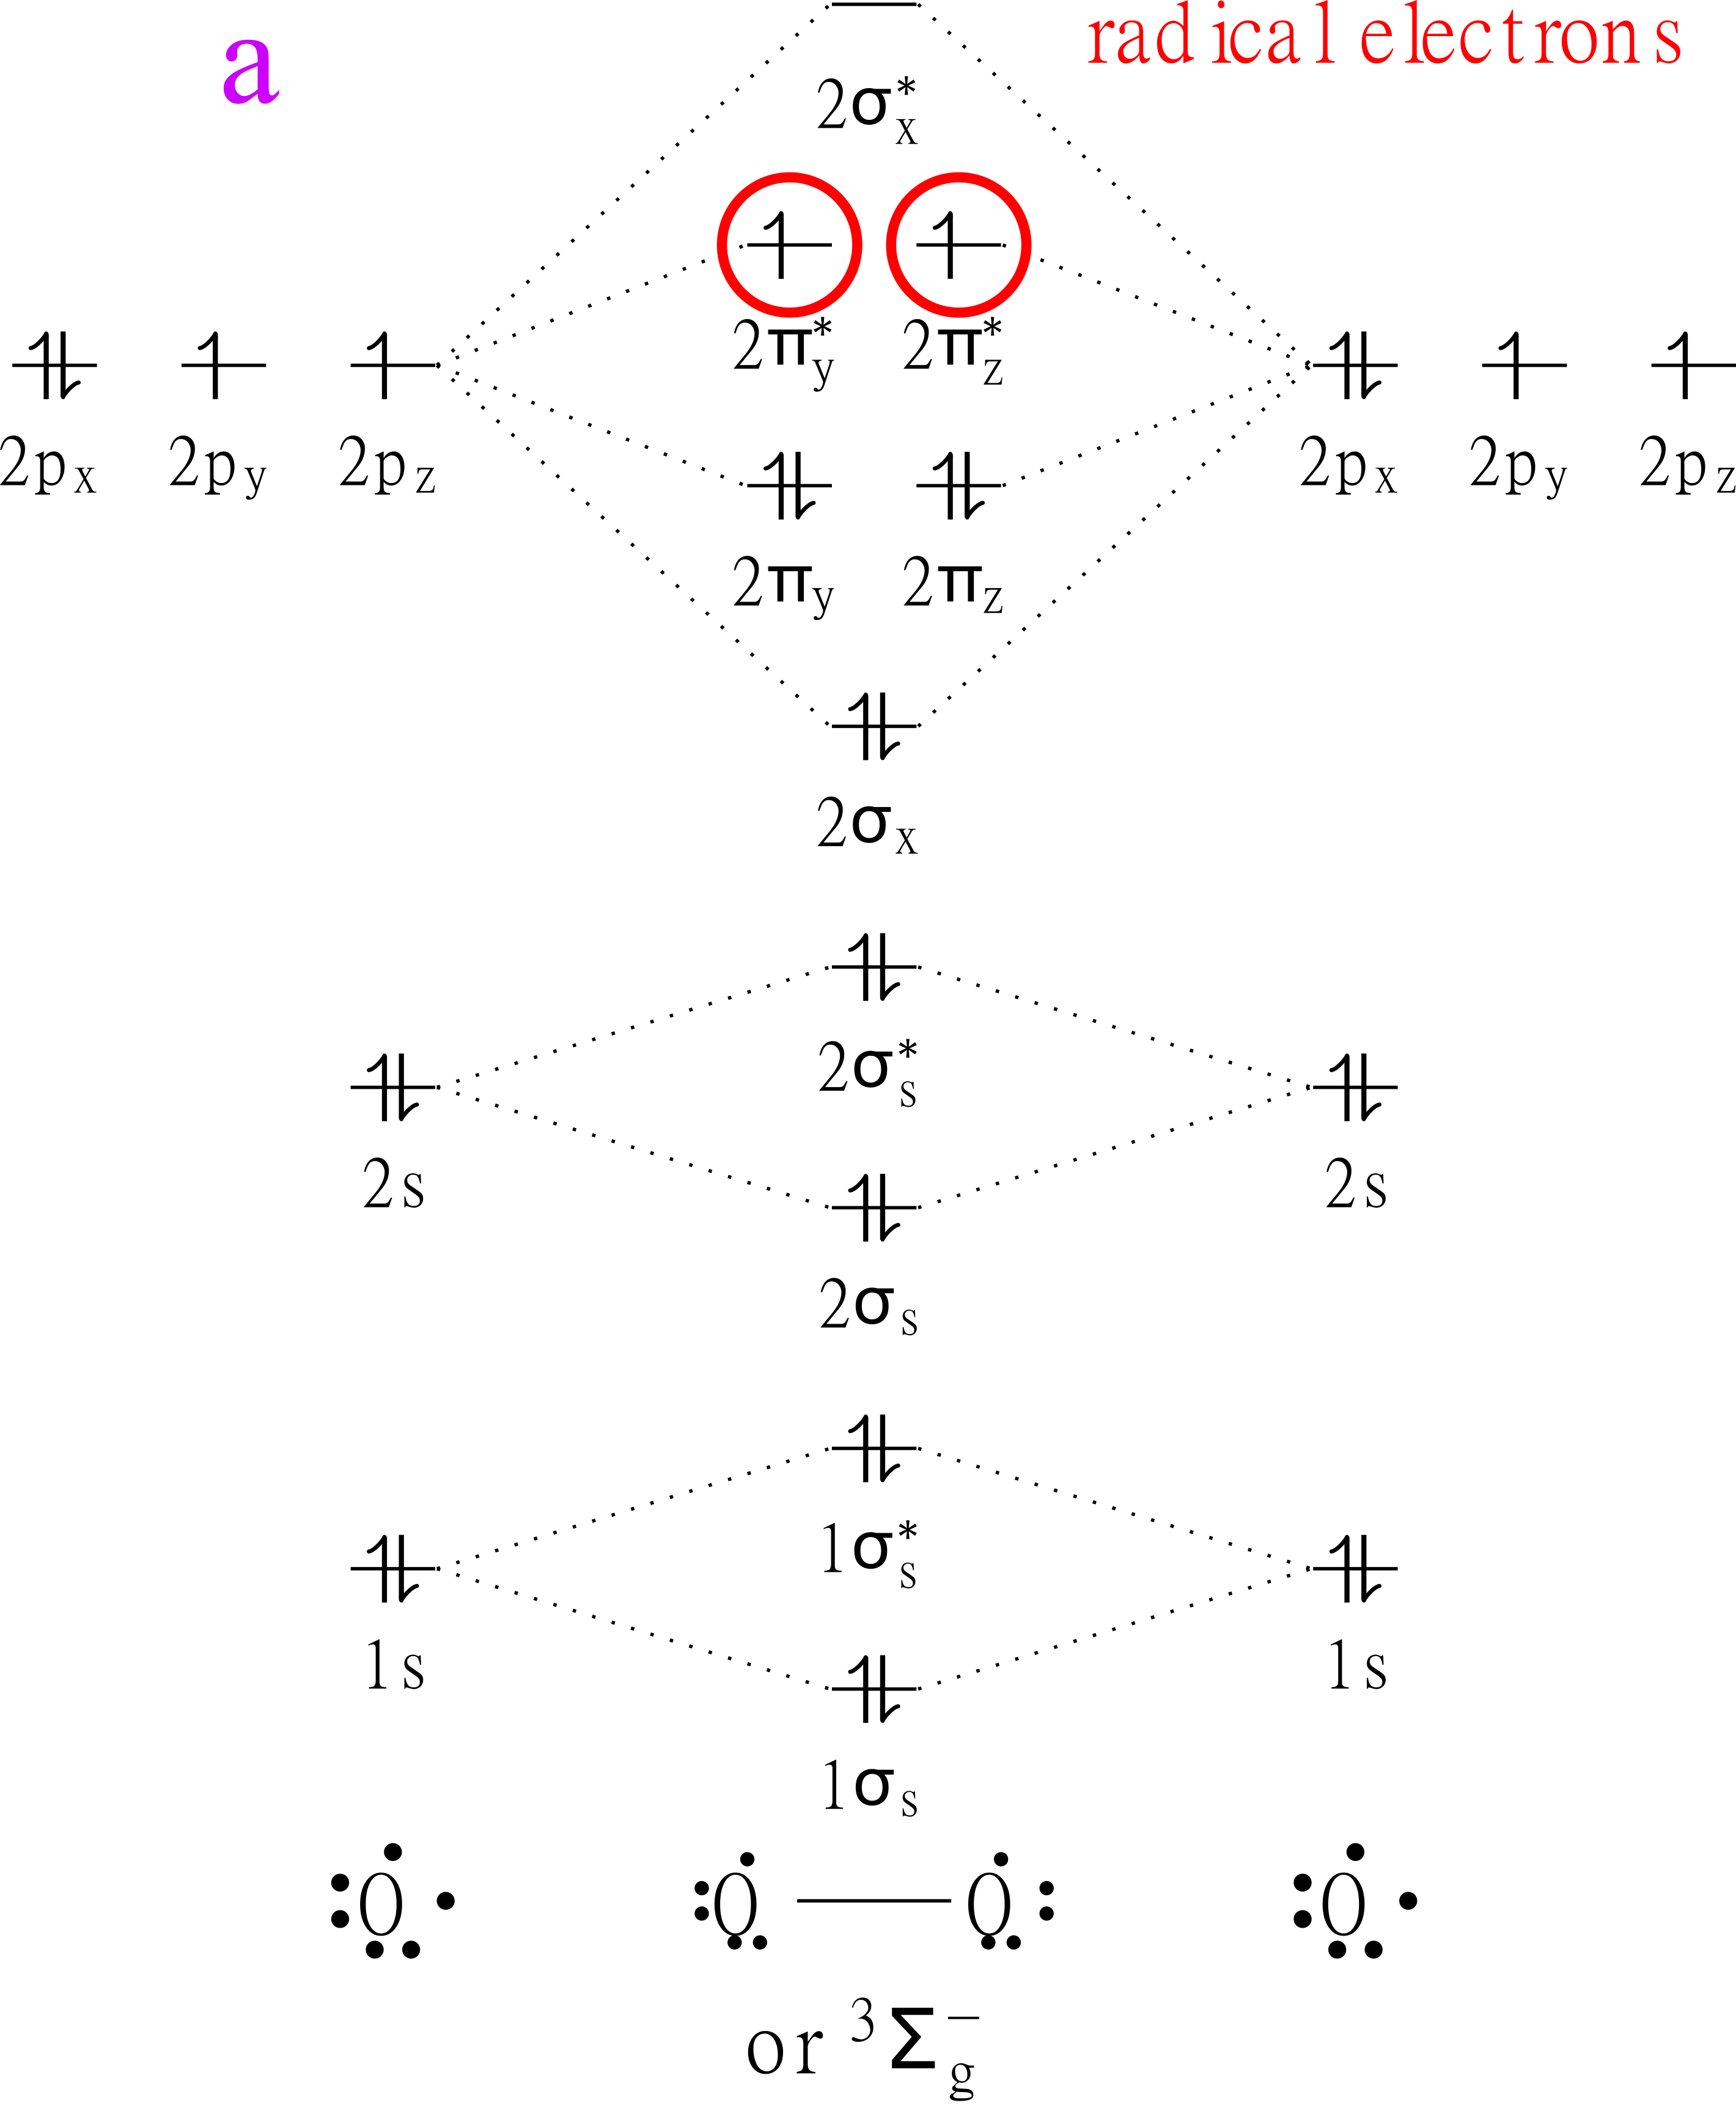
\includegraphics[width = 0.48\textwidth]{images/PDIpy/background/triplet_mo_diagram.png}
        & 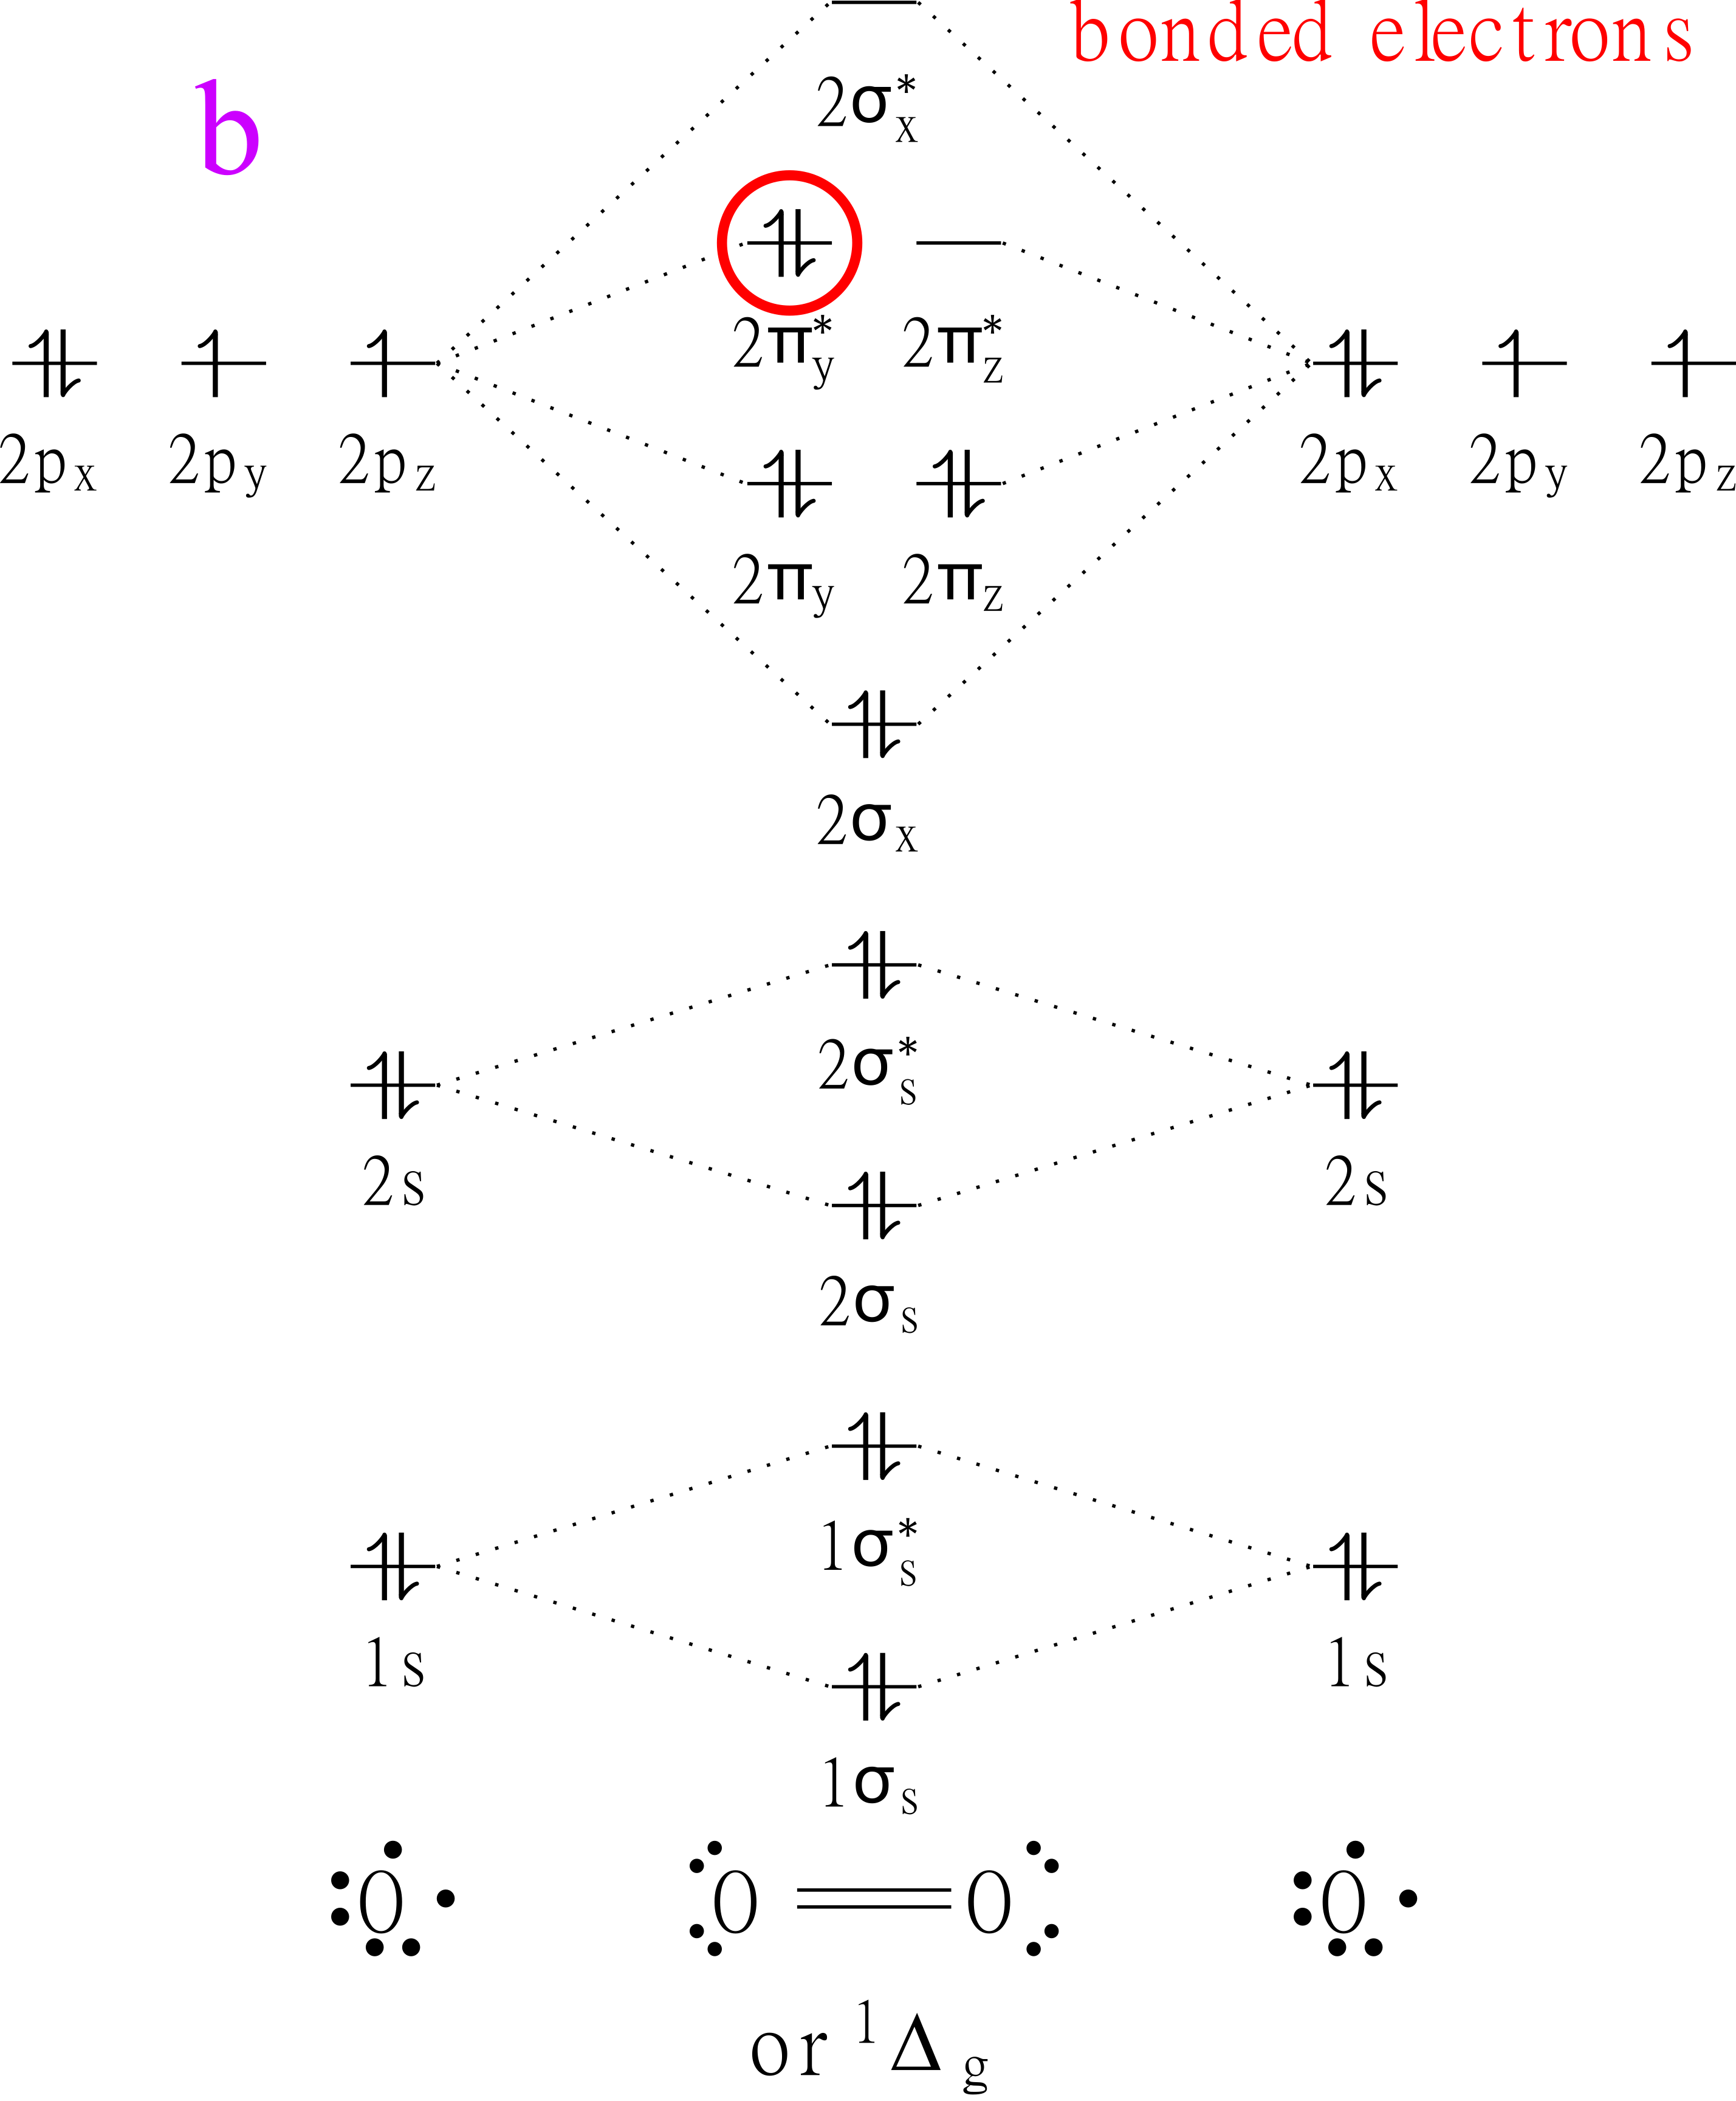
\includegraphics[width = 0.48\textwidth]{images/PDIpy/background/singlet_mo_diagram.png}
    \end{tabular}
    \caption{
        Qualitative orbital diagrams for a) $^3\Sigma_g^-$ and b) $^1\Delta_g$ configurations of diatomic oxygen. Each barbed arrow represents a single electron, and each platform represents the electronic sub-orbital of the respective label, where orbital energy increases vertically in the diagram. The distinction between a) and b) is highlighted by the red circled electrons and labels, where $^1\Delta_g$ possesses an anti-bonding $\pi^*$-bond in its HOMO that destabilizes it relative to $^3\Sigma_g^-$.
    }
    \label{mo_diagrams}
\end{figure}

\begin{figure}[t]
    \centering
    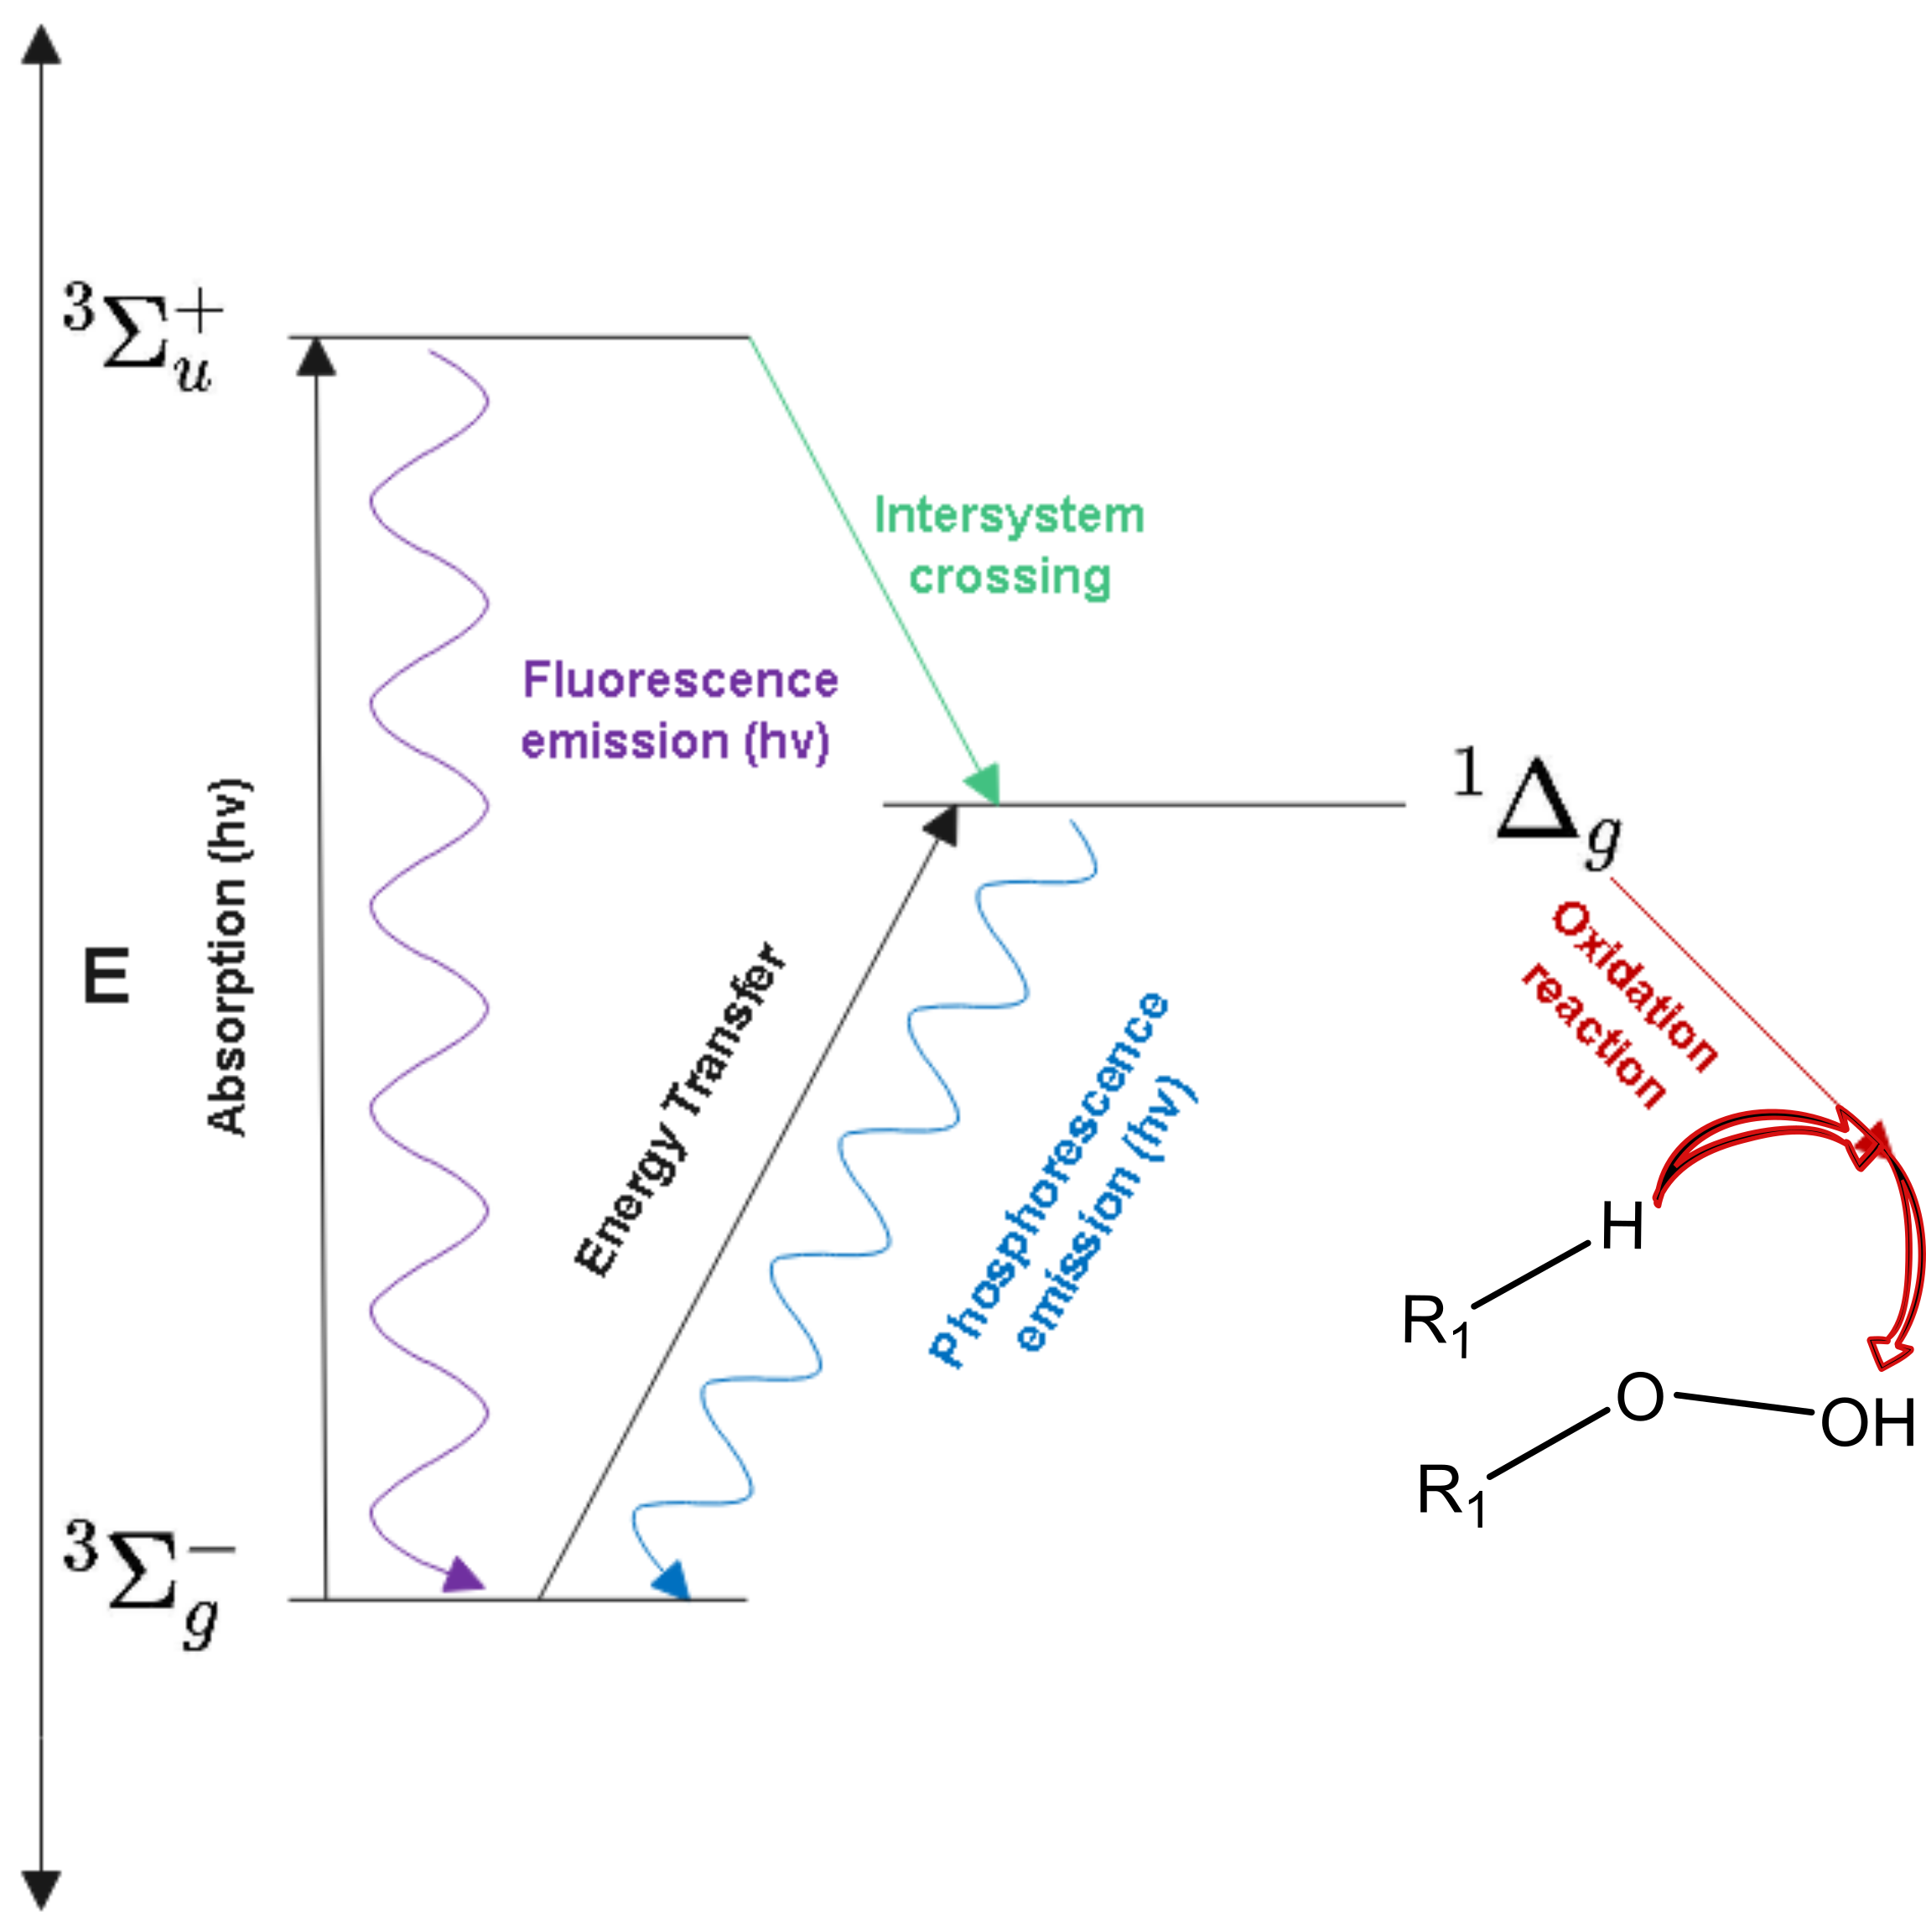
\includegraphics[width = \textwidth]{images/PDIpy/background/jablonski_diagram.png}
    \caption{
        A qualitative Jablonski energy diagram of Steps b-c of PDI. The initial excitation in PDI occurs via an energy transfer $\ce{^3\Sigma_g^- ->[energy transfer] ^1\Delta_g}$. The ROS then, while abstaining from phosphoresce, oxidizes a biological substrate to form a peroxide that gradually compounds to cause lysis.
    }
    \label{jablonski_diagram}
\end{figure}

\begin{figure}[t]
    \centering
    \includegraphics[width = \textwidth]{images/PDIpy/background/BCFA_schenck_oxidation_2.png}
    \caption{
         The reaction mechanisms of Type II oxidation and subsequent decompositions. \textbf{Step (1)} depicts the concerted \cite{Foote1968PhotosensitizedOxygen} Schenck reaction. \textbf{Step (2)} depicts the homolytic cleavage of the hydroperoxide bond to form $\ce{OH^.}$ and an oxy radical that may enter autoxidation (Type I oxidation) mechanisms. \textbf{Step (3)} depicts radical propagation via hydrogen abstraction to form another radical substrate and an alcohol byproduct. \textbf{Step (4)} is a concerted Russell reaction \cite{Russell1957Deuterium-isotopeRadicals,Howard1968TheMechanism} between two peroxides that forms a $\ce{H2O2}$, an $\alpha,\beta$-ketone, and an alcohol. The reactions of Steps (2-4) sample the wide range of possible decompositions that follow oxidation mechanisms.
    }
    \label{schenck_mechanism}
\end{figure}

\subsection{Excitation proportion} \label{excitation_proportion_estimate}

The steps for estimating the absorbed proportion of incident photons by photosensitizers, where absorbance or transmittance measurements are not available, are detailed through the following steps. a) The reported intensity of incident light from the respective light source -- i.e. irradiance ($\frac{mW}{cm^2}$), lux ($\frac{lumen}{m^2}$), or lumens (lumens) -- is converted into a quantity of incident watts $watts_{in}$ ($\frac{J}{s}$). b) This incident wattage is attenuated by the proportion of the emission spectra $spec_{em}$ that resides within the $spec_{ex}$ of the PS, 
\begin{equation}
    watt_{ex} = \frac{spec_{ex}}{spec_{em}}*watts_{in}.
\end{equation}
c) The $watt_{ex}$ is then used to calculate the moles of incident photons that strike photosensitizers per timestep 
\begin{multline} \label{photons_per_second}
    \frac{photons_{strike~PS}}{timestep}=\frac{<h\nu_{ex}>}{h*c}*watts_{ex} *\frac{s}{\Delta t}*reflection*scattering*\frac{1~mole}{N_A}*\frac{vol_{PS}}{vol_{total}},
\end{multline}
where $reflection \approx 96 \%$ and represents the proportion of incident photons that penetrate an aqueous solution \cite{Gross1993SingletLiposomes}; and $scattering \left(\frac{I_z}{I_0} = e^{-k*z}\right)$ represents the proportion of light $\frac{I_z}{I_0}$ that reaches a specified depth $z$ \cite{RobertW.1973TheSea}, where $k$ is the attenuation coefficient that is $\approx 0.04~(\frac{1}{m})$ \cite{Lorenzen1972ExtinctionPhytoplankton} for clear water. The quotient $\frac{vol_{PS}}{vol_{total}}$ describes the fraction of the solution volume where the PS resides ($vol_{total}$) that is comprised of the PS per se ($vol_{PS}$), which is calculated as the product of the quantity of PS molecules and the volume per molecule according to its molecular structure. The average excitation wavelength of the PS ($<h\nu_{excitation}>$) is calculated as the weighted average of the Soret and Q excitation bands, in proportion to their relative contribution in generating $^1\Delta_g$ \cite{Nitzan2001PhotoinactivationWavelengths,Hoenes2020PhotoinactivationWavelength}, which assumes that both excitation wavelengths are excited during the simulation. The resultant $\frac{photons_{strike~PS}}{timestep}$ from \cref{photons_per_second} is then divided by the quantity of photons that enter the system per timestep $\frac{photons_{total}}{timestep}$ to determine which fraction of photons strike a photosensitizer. 

\subsection{Deduction of inactivation via the Hill equation}

Inactivation may alternatively be deduced from oxidation through parameter manuipulation of a fitted sigmoidal curve, similar to other models \cite{Xiong1999AInactivation}. The Hill-equation \cite{Gesztelyi2012ThePharmacology} is a sigmoidal model that derives from mass-action kinetics, similar to the Michaelis-Menten kinetic model, and thus it was selected the signmoidal model for this alternative framework. A Python program for fitting the Hill-equation was developed -- the HillFit module -- with a variation of the Hill-equation \cite{Inoue2016OscillationActivation} 
\begin{equation} \label{hill_eq}
    y=bottom+\frac{(top-bottom)*x^n}{EC50^n+x^n},
\end{equation}
that introduces an additional $bottom$ parameter for more advantageous fitting. The predicted oxidation data was fitted to a hill-equation via HillFit and the parameters were subsequently adjusted in Table \ref{hill_parameters} to optimally meet the training data. The $top$ parameter of \cref{hill_eq} is adjusted asymptotically to a limit that follows an subtly different empirical expression for planktonic $1-10^{-\Omega}$ than biofilm $1-10^{-0.7-\Omega }$ simulations, where $\Omega = wattage^{\frac{1}{5}}-log10(1-final_{oxidation\_proportion})$. This limit manifests in the predicted inactivation being $\approx [1,2]-log$ greater than the predicted oxidation, which implicitly specifies an oxidation thereshold of $\approx [1,10]\%$. The different parameter adjustments between sessile and planktonic systems may be explained that numerous chemical influences, such as diffusion rates, are not explicitly considered in our kinetic model. The regression plots for the fit of the Beirao et al. training data is depicted in Figure \ref{hill_regression}. The very precise fitting -- $R^2 > 0.996$ -- supports that the Hill-equation is an accurate description of our kinetic PDI model, and conversely that our model fundamentally describes a biochemical relationship.

\begin{figure}
    \centering
    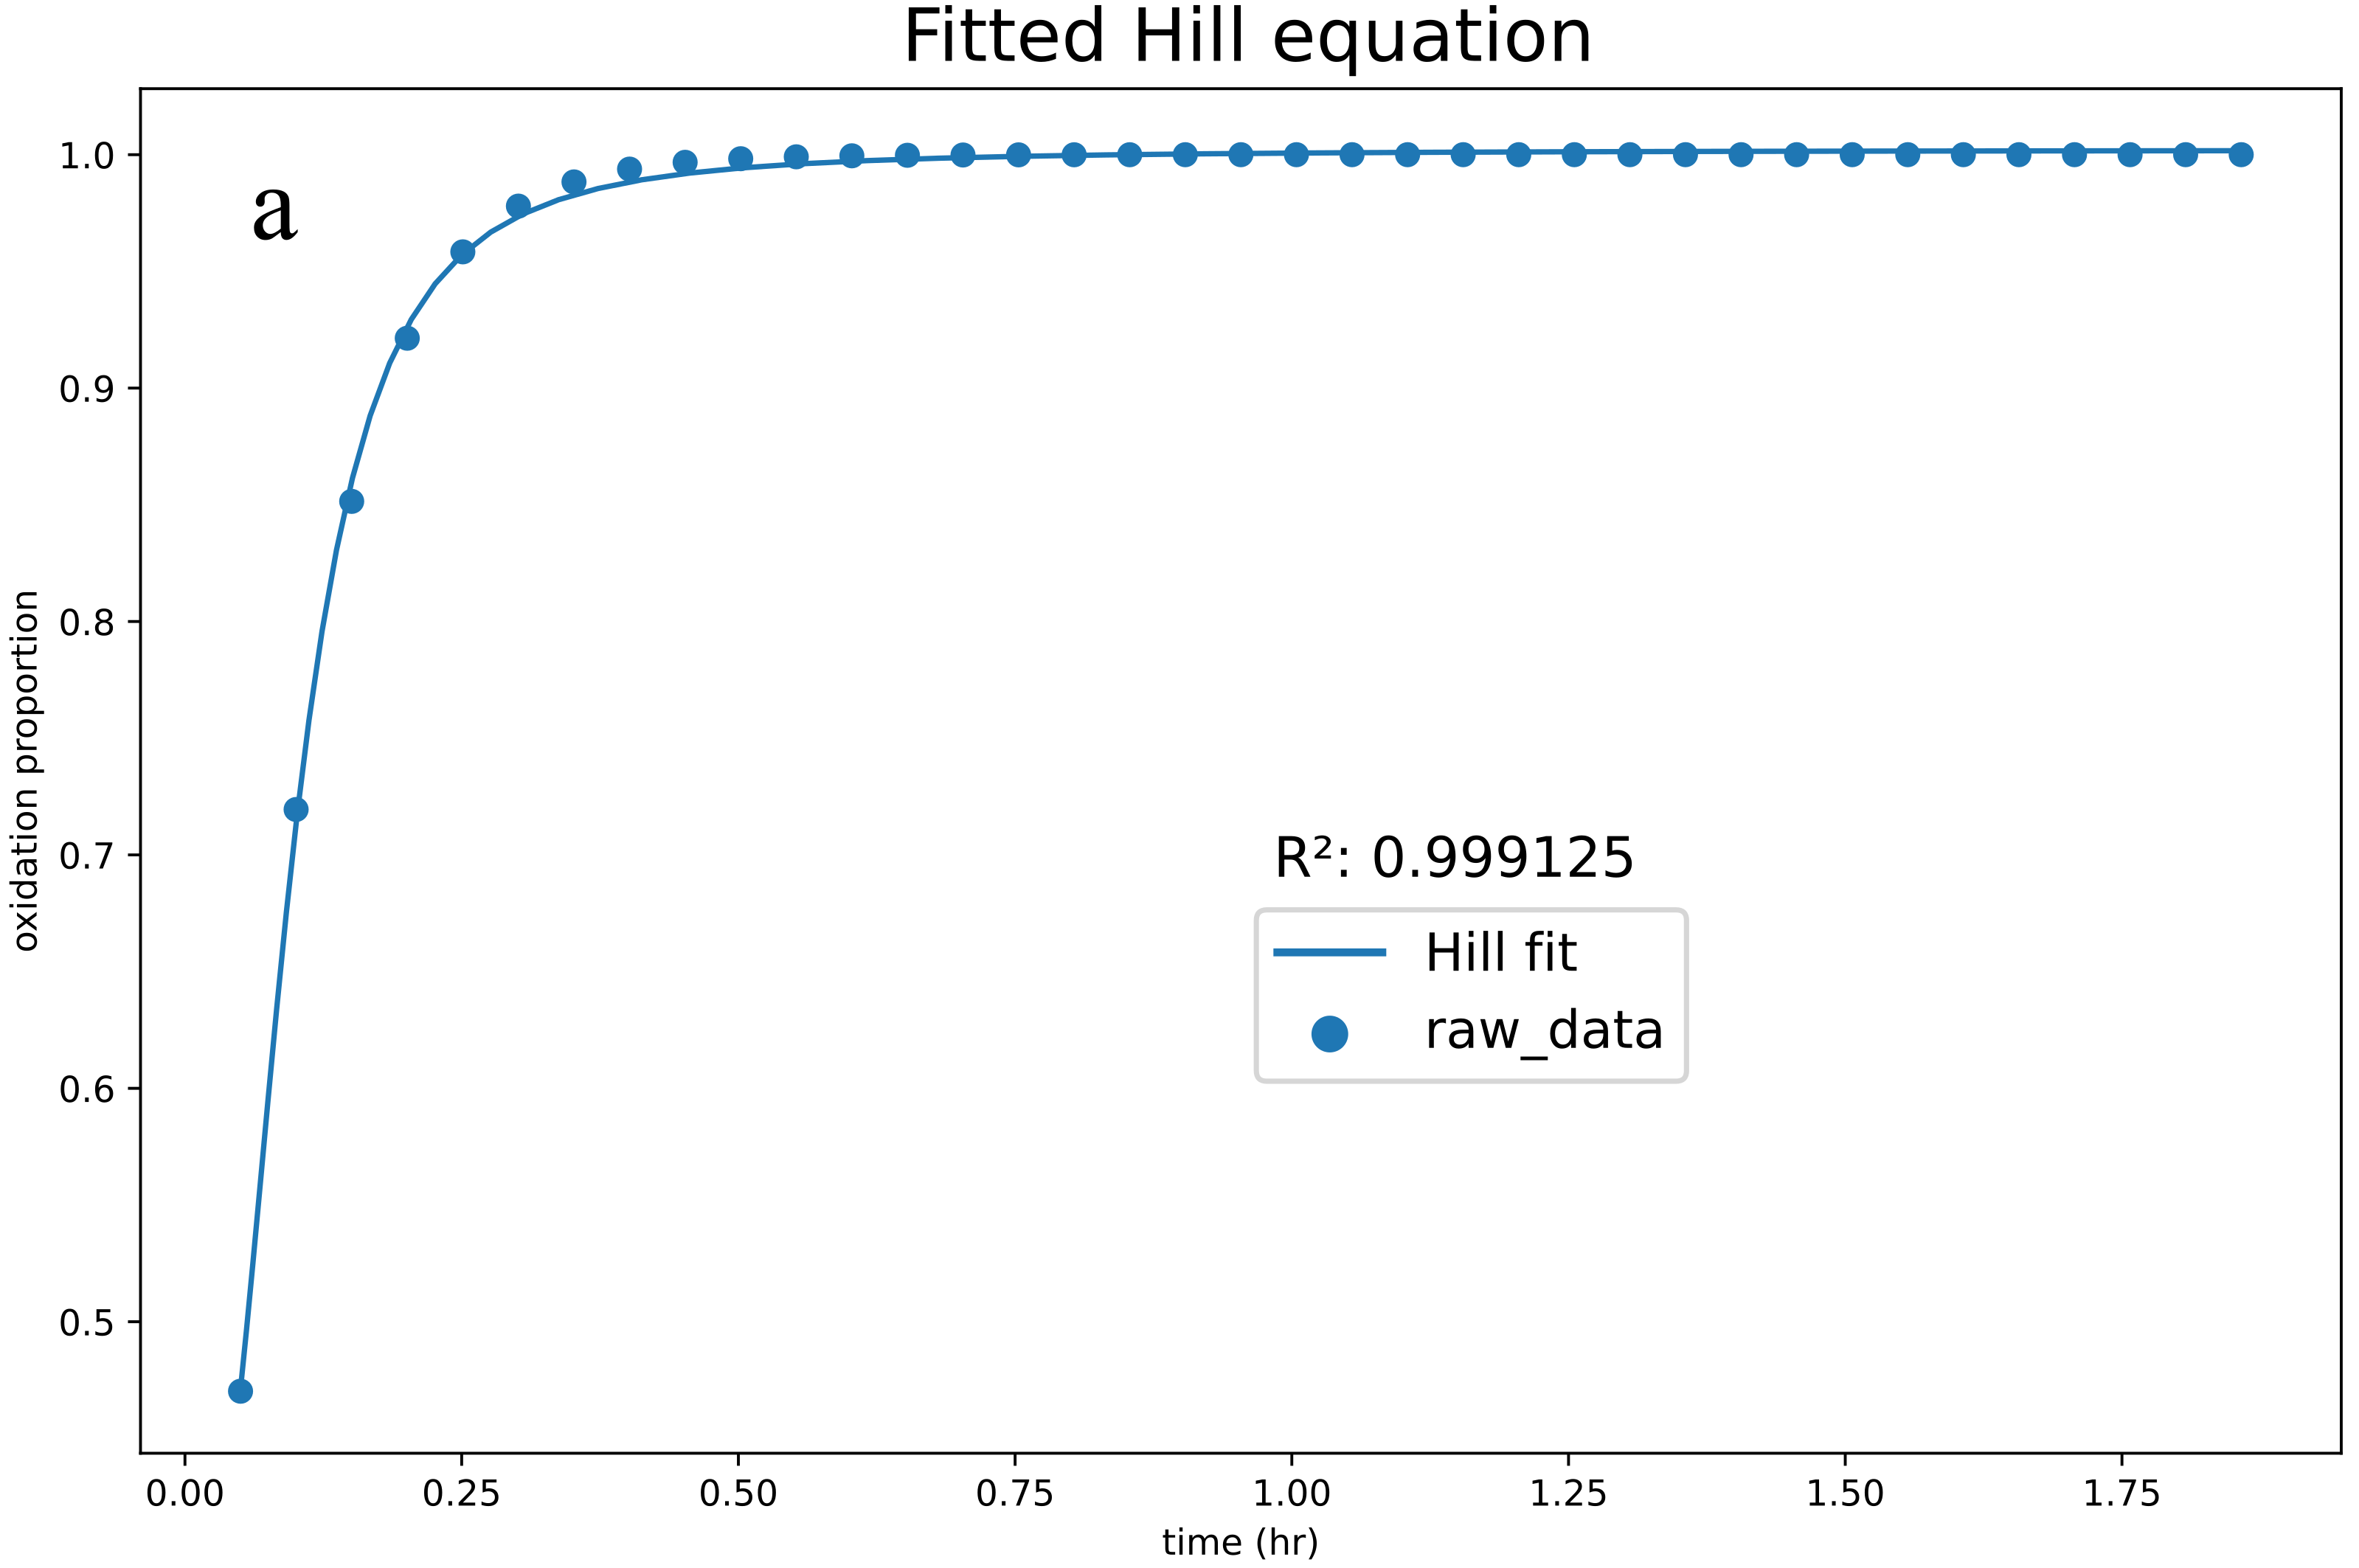
\includegraphics[width = 0.9\textwidth]{images/PDIpy/training/10uM_regression.png}
    \vspace{5mm}
    \midrule
    \vspace{5mm}
    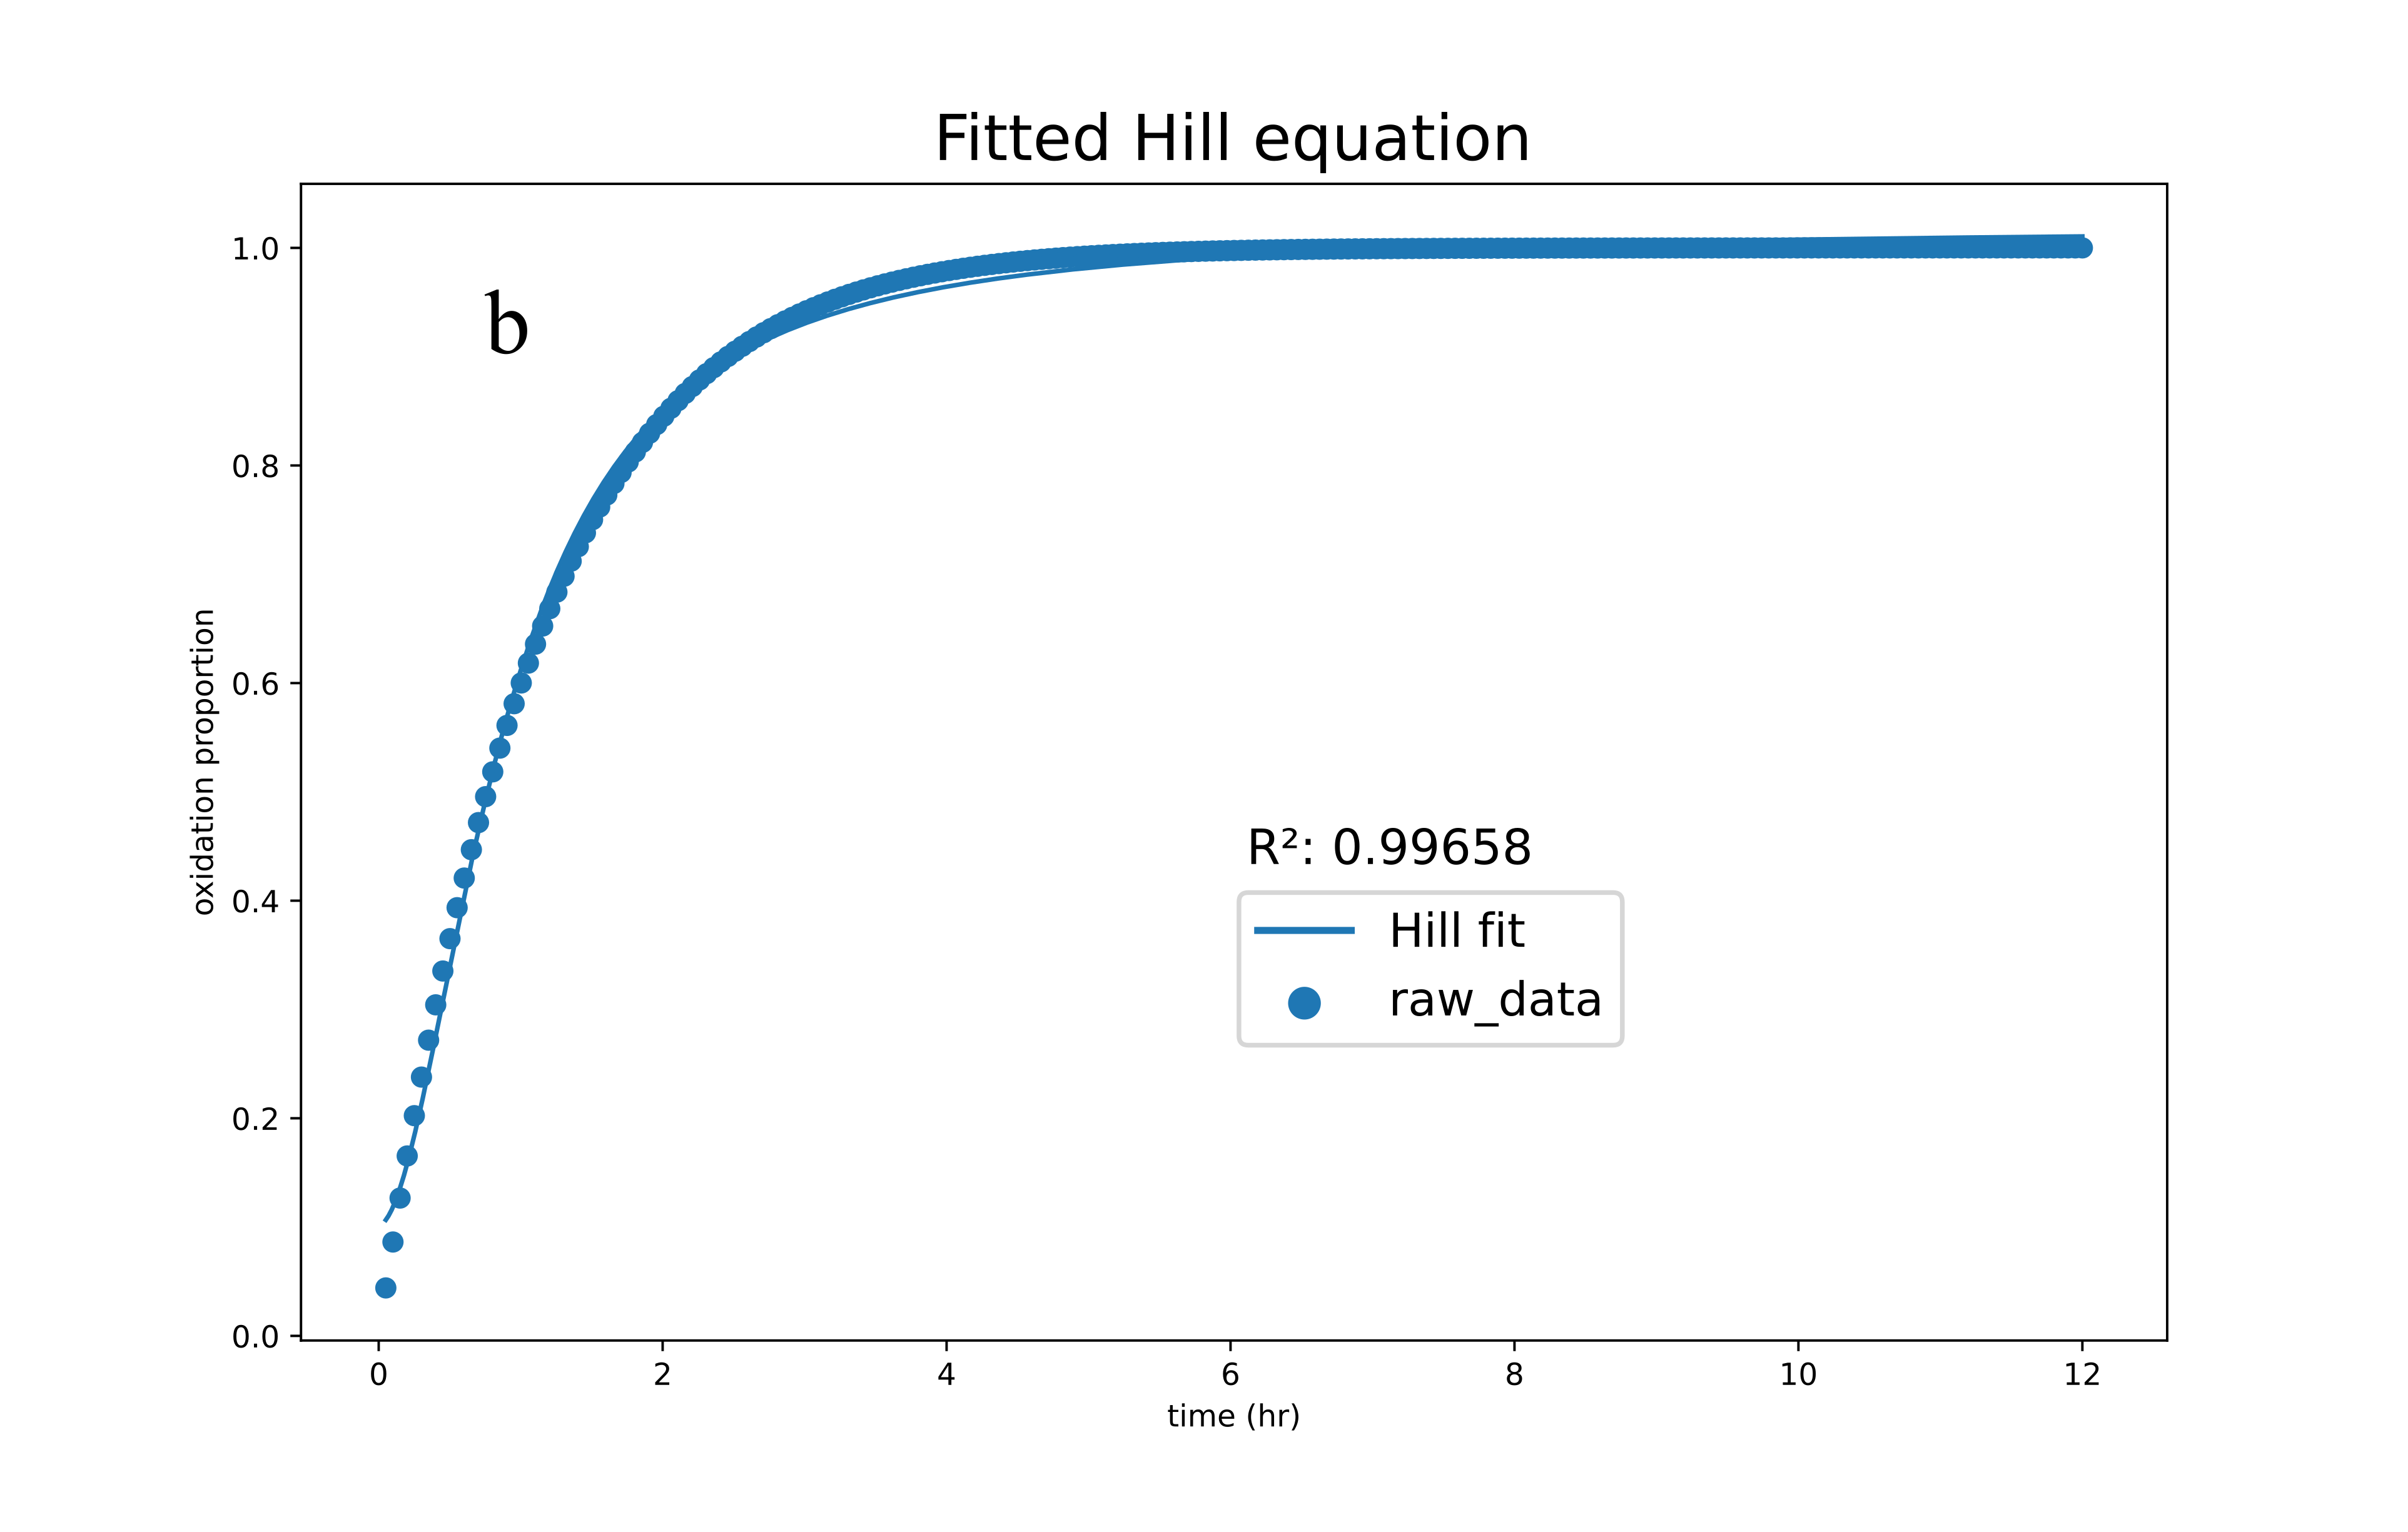
\includegraphics[width = 0.9\textwidth]{images/PDIpy/training/10uM_biofilm_regression.png}
    \caption{
        The Hill-equation regressions for the oxidation plots of the Beirao et al. training data for a) planktonic and b) sessile states. The high $R^2$ correlation supports that our chemical model of PDI recreates a sigmoidal biochemical relationship. The greater number of data points in panel b) is the consequence of a far longer simulation time than the simulation of panel a).
    }
    \label{hill_regression}
\end{figure}

% \begin{table}
%     \centering
%     \begin{tabular}{l|c|c}
%         \textbf{Bacterial state} & \textbf{Hill parameter} & \textbf{Adjustment} \\
%         \multirow{2}{}{Planktonic} & EC50 & -76\% \\
%          & nH & +100\% \\
%     \end{tabular}
%     \caption{
%         The Hill parameters adjustments that are enacted to create the inactivation plot for simulations of planktonic systems. 
%     }
%     \label{hill_parameters}
% \end{table}

\subsection{Oxidized membrane region}
The region of the bacterial membrane that is oxidized by cross-linked PSs may be a small fraction of the total membrane, provided that the bacterium does not have a tremendous angular momentum. This is not presently captured by our model, but the following logic could incorporate this concept into the model. The oxidized region of a coccus bacterial cell can be determined from the cellular radius and volume
\begin{equation}
    radius_{cell} = \sqrt[3]{3*\frac{volume_{cell}}{4\pi}}~.
\end{equation}
The membrane volume is calculated
\begin{equation}
    volume_{membrane} = \frac{4\pi}{3}*(radius_{cell}^3 - (radius_{cell}-th_{membrane})^3)
\end{equation}
there the thickness of the cytoplasmic membrane $\approx 4 nm$. The volume of oxidized membrane is then calculated
\begin{equation}
    volume_{oxidized} = volume_{membrane}*\frac{angle_{oxidized}}{360}~,    
\end{equation}
where the $angle_{oxidized}$ describes the angle in degrees from vertical at which the farthest $^1\Delta_g$ reaches the mebrane. The fraction of the membrane volume that is oxidized is then calculated 
\begin{equation}
    oxidized = \frac{volume_{oxidized}}{volume_{membrane}} 
\end{equation}
and applied to augment the effective oxidation proportion
\begin{equation}
    oxidation_{proportion,new} = \frac{oxidation_{proportion,old}}{oxidized}~.
\end{equation}

\subsection{Sensitivity analyses}

\paragraph{Light source \& emission}
The sensitivity of simulation results to the light source -- incandescent, LED, or fluorescent -- was explored. The comparison of incandescent and LED light sources, where LED and fluorescent were nearly indistinguishable, is depicted in Figure \ref{light_source}. These simulated differences are solely attributed to differences in the proportion of emitted photons that are within the visible spectrum, since PDIpy does not current resolve the intensity of specific emitted wavelengths or consider the inactivation effects of heat from incandescent bulbs. The visible proportion of the emitted wavelengths was determined in Figure \ref{light_emission} to have minimally consequence above 20\%.

\begin{figure}
    \centering
    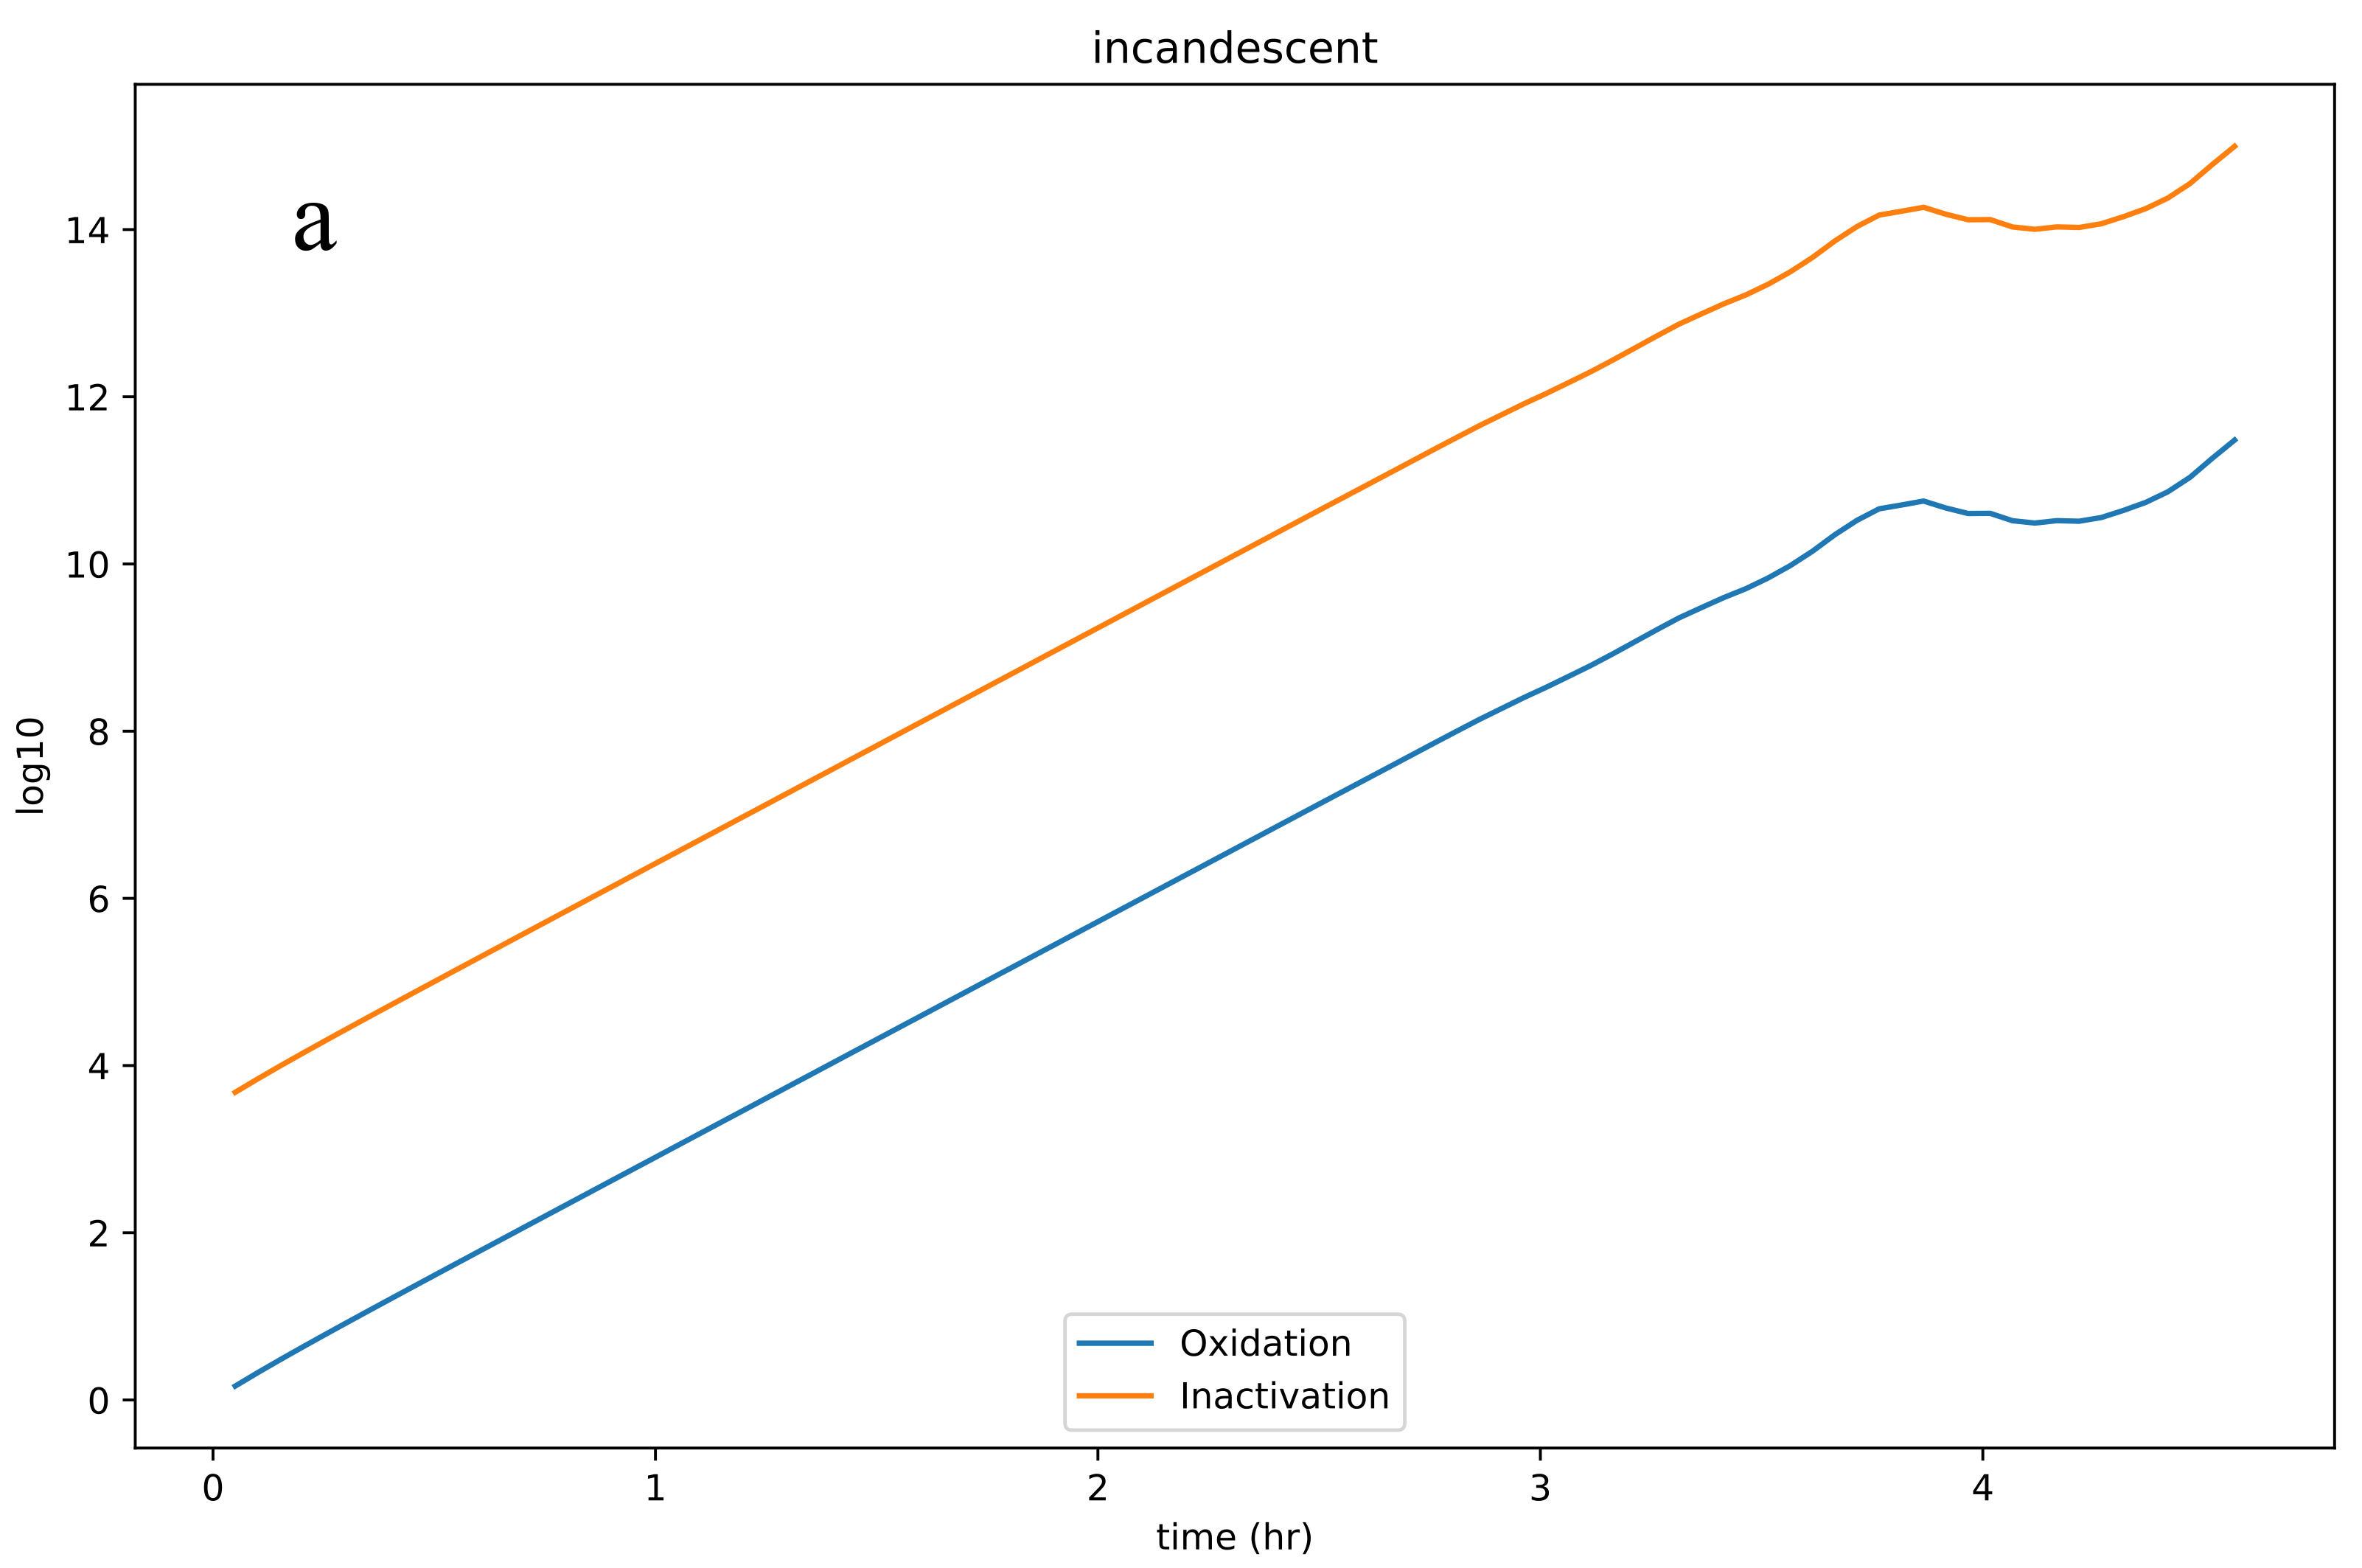
\includegraphics[width = 0.9\textwidth]{images/PDIpy/sensitivity_analyses/light_source/incandescent.png} \\
    \vspace{5mm}
    \midrule
    \vspace{5mm}
    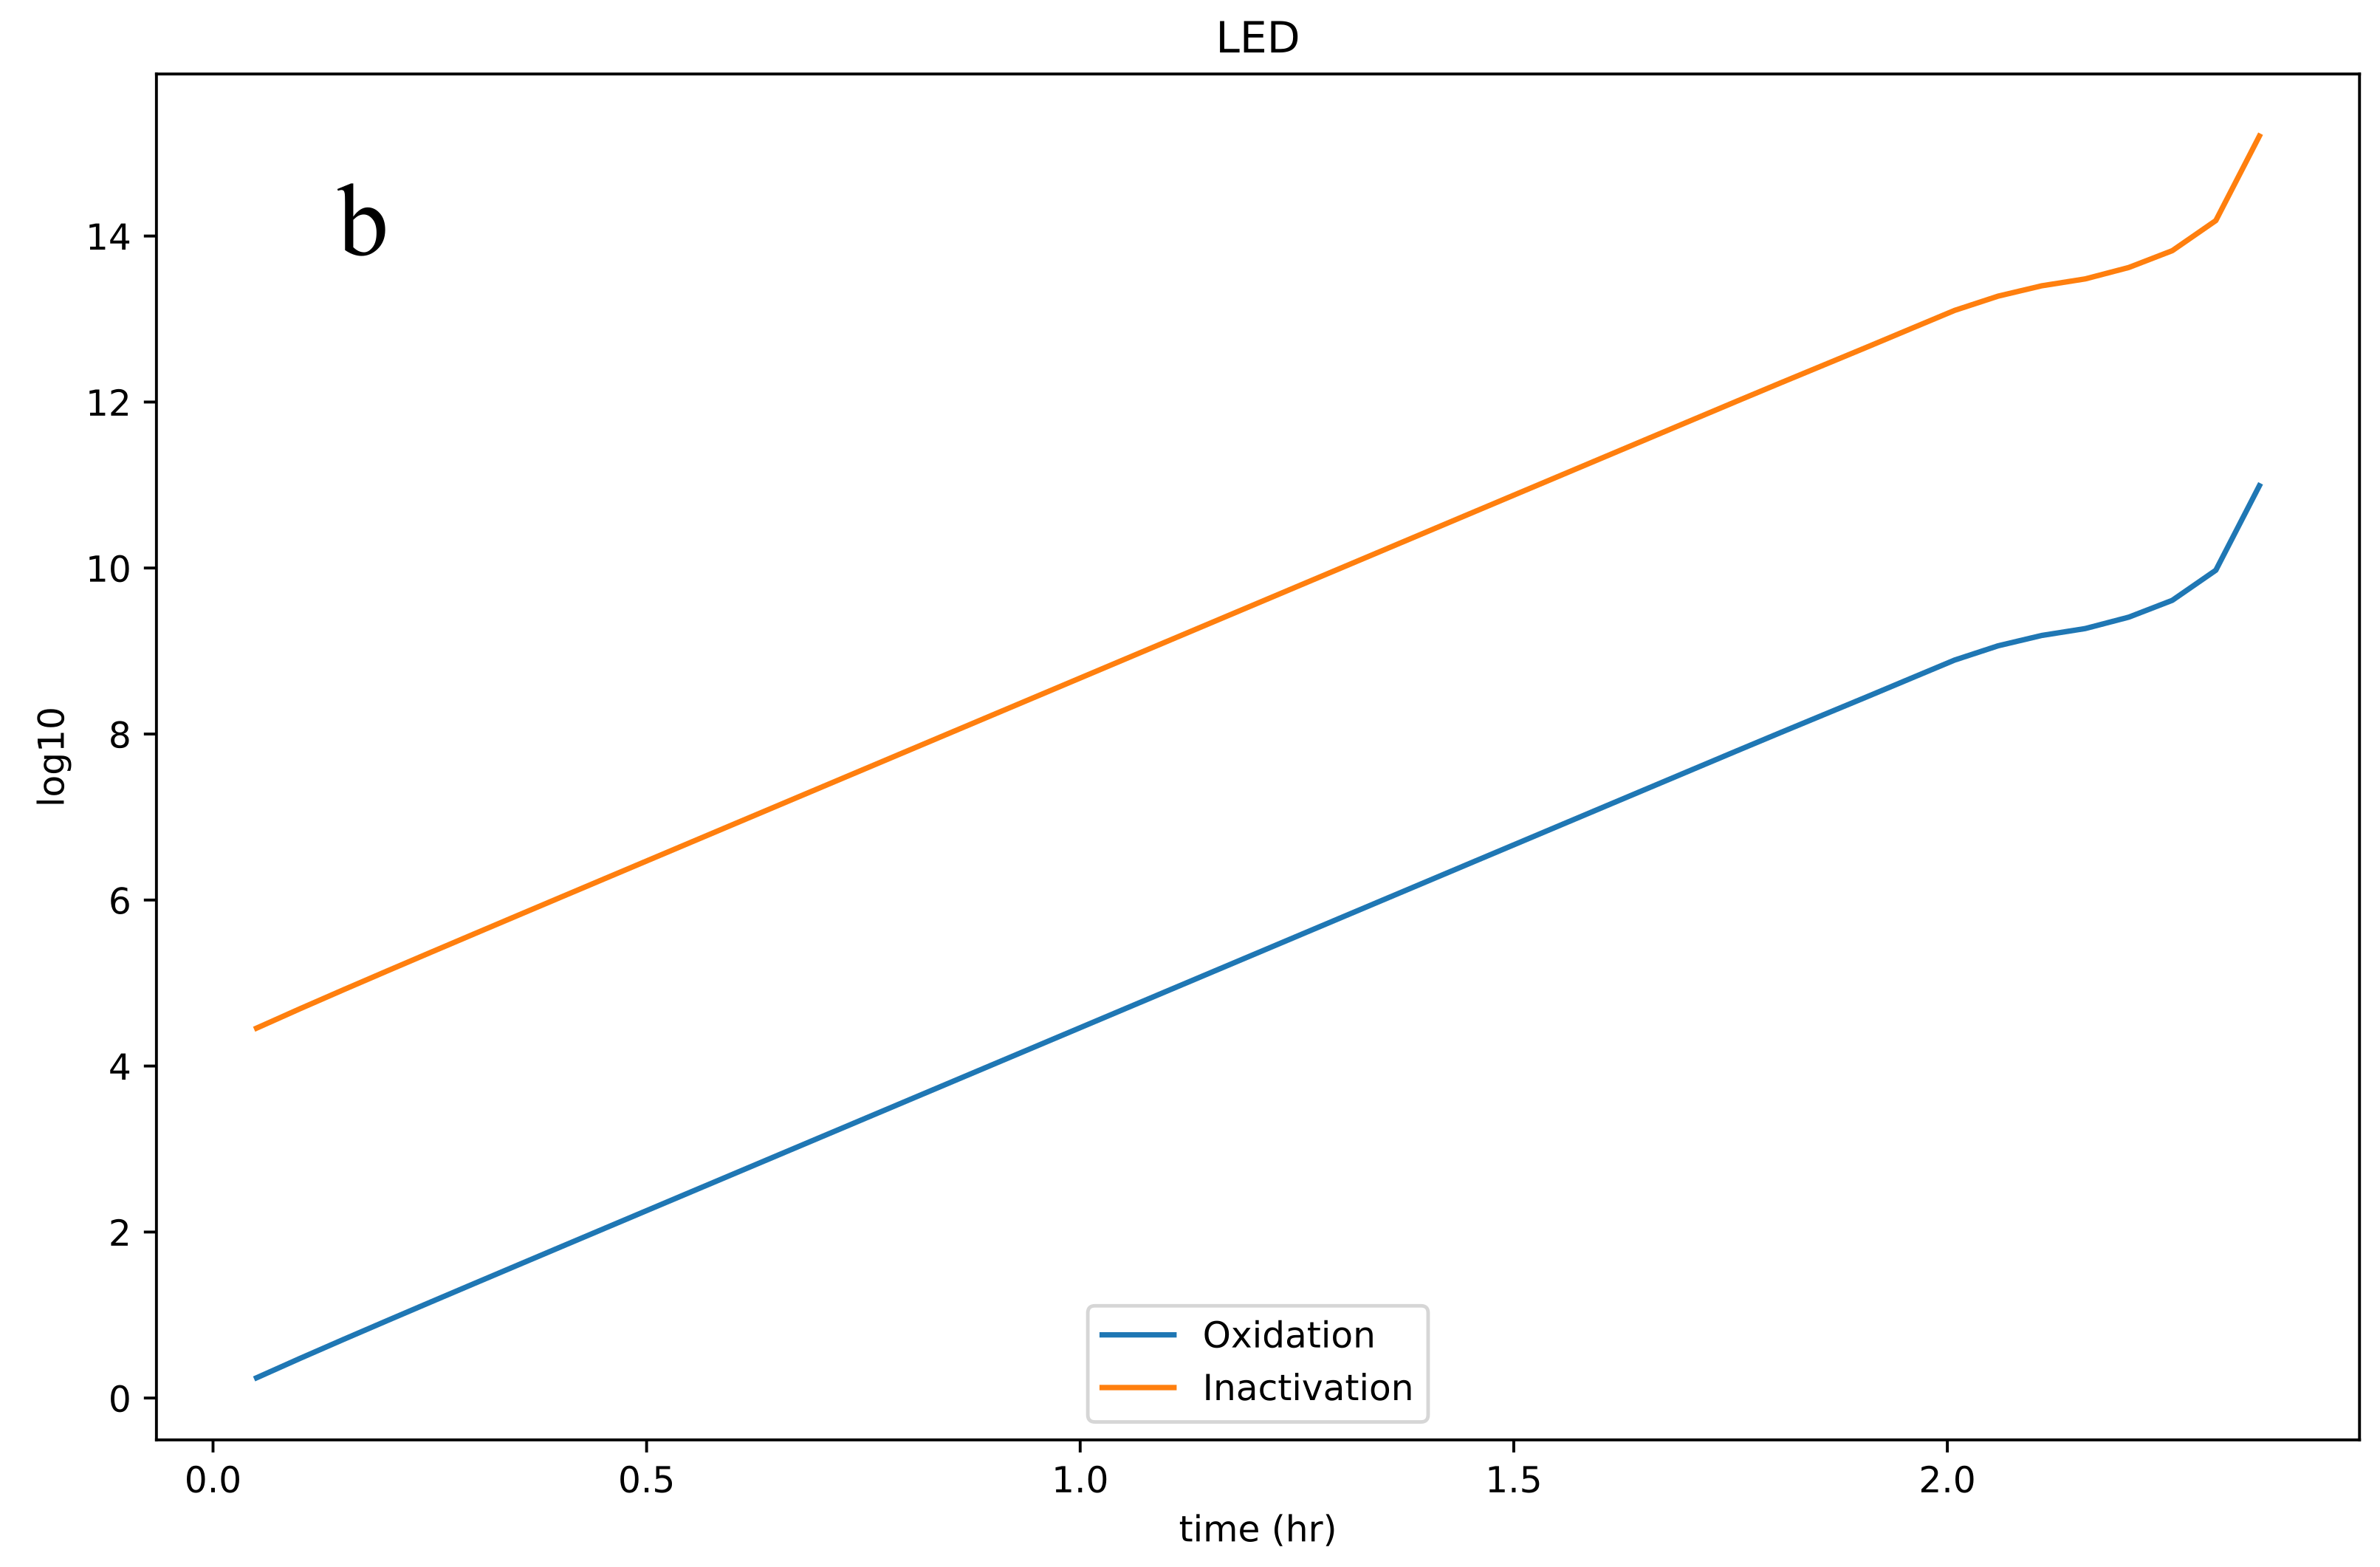
\includegraphics[width = 0.9\textwidth]{images/PDIpy/sensitivity_analyses/light_source/LED.png}
    \caption{
        A comparison of the same experiment under a) incandescent and b) LED light sources. The discrepancy between the inactivation of the two sources is attributed to the proportion of emission that resides in the visible spectrum.
    }
    \label{light_source}
\end{figure}

\begin{figure}
    \centering
    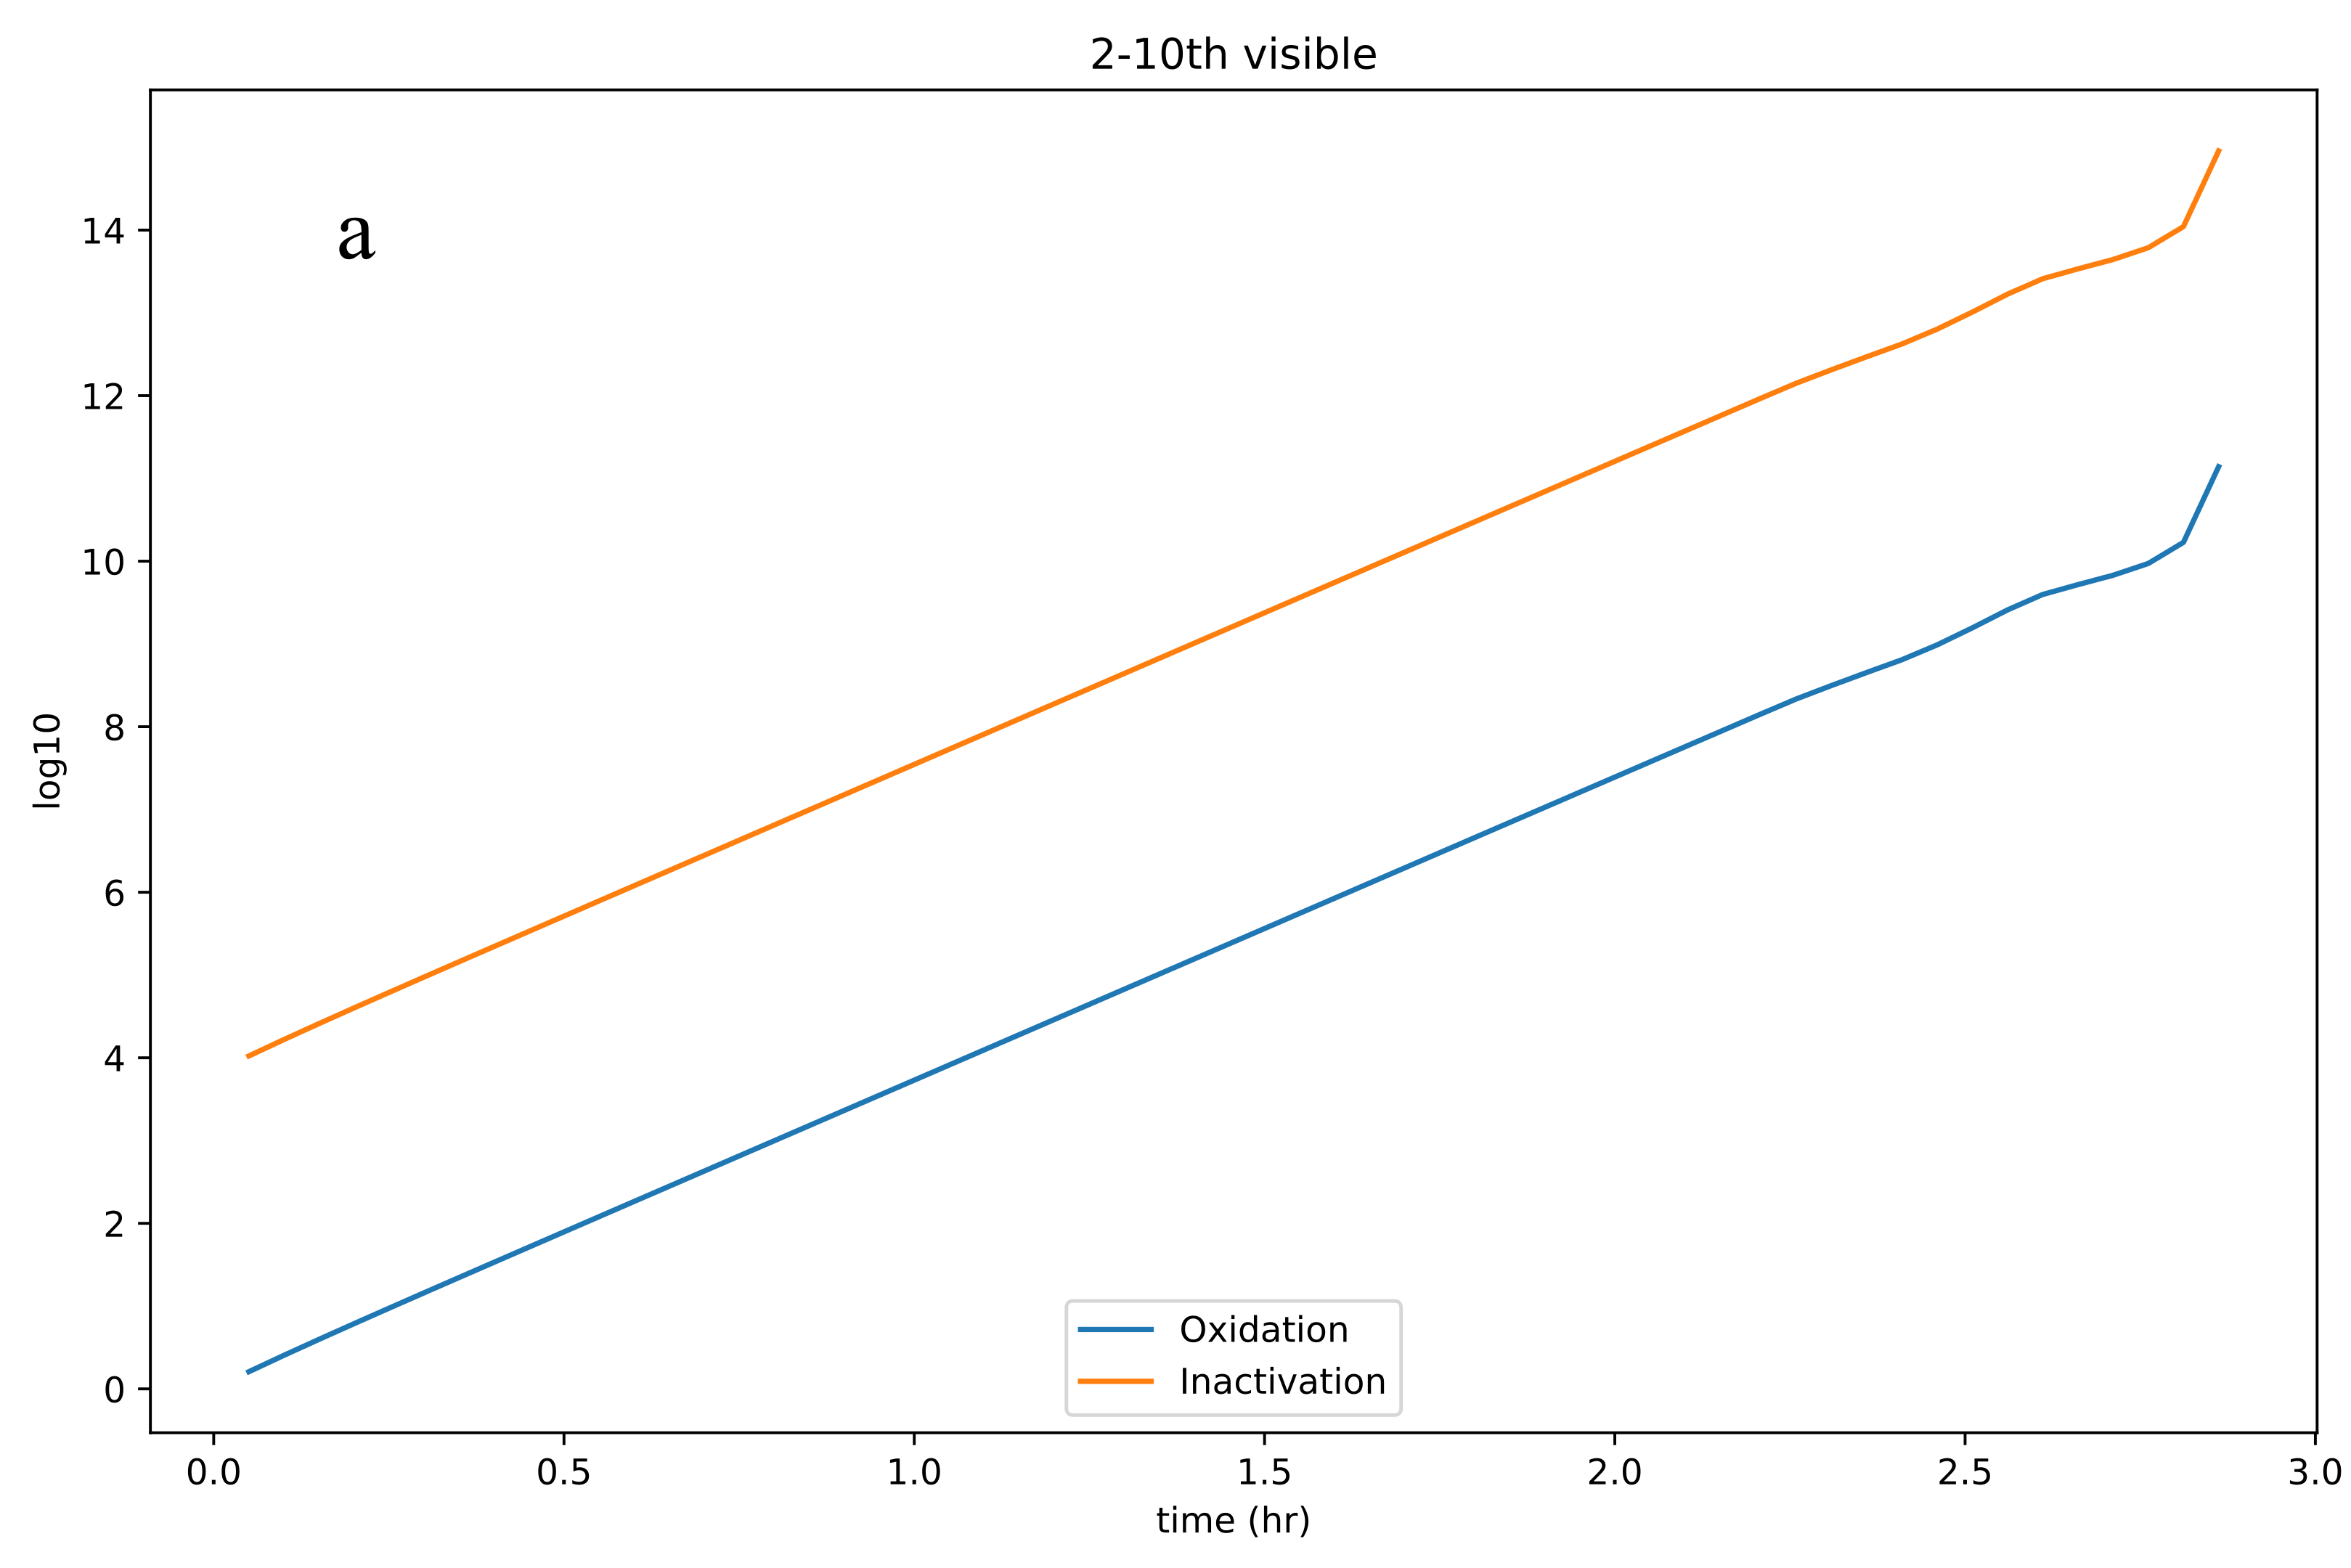
\includegraphics[width = 0.9\textwidth]{images/PDIpy/sensitivity_analyses/light_emission/20_visible.png} \\
    \vspace{5mm}
    \midrule
    \vspace{5mm}
    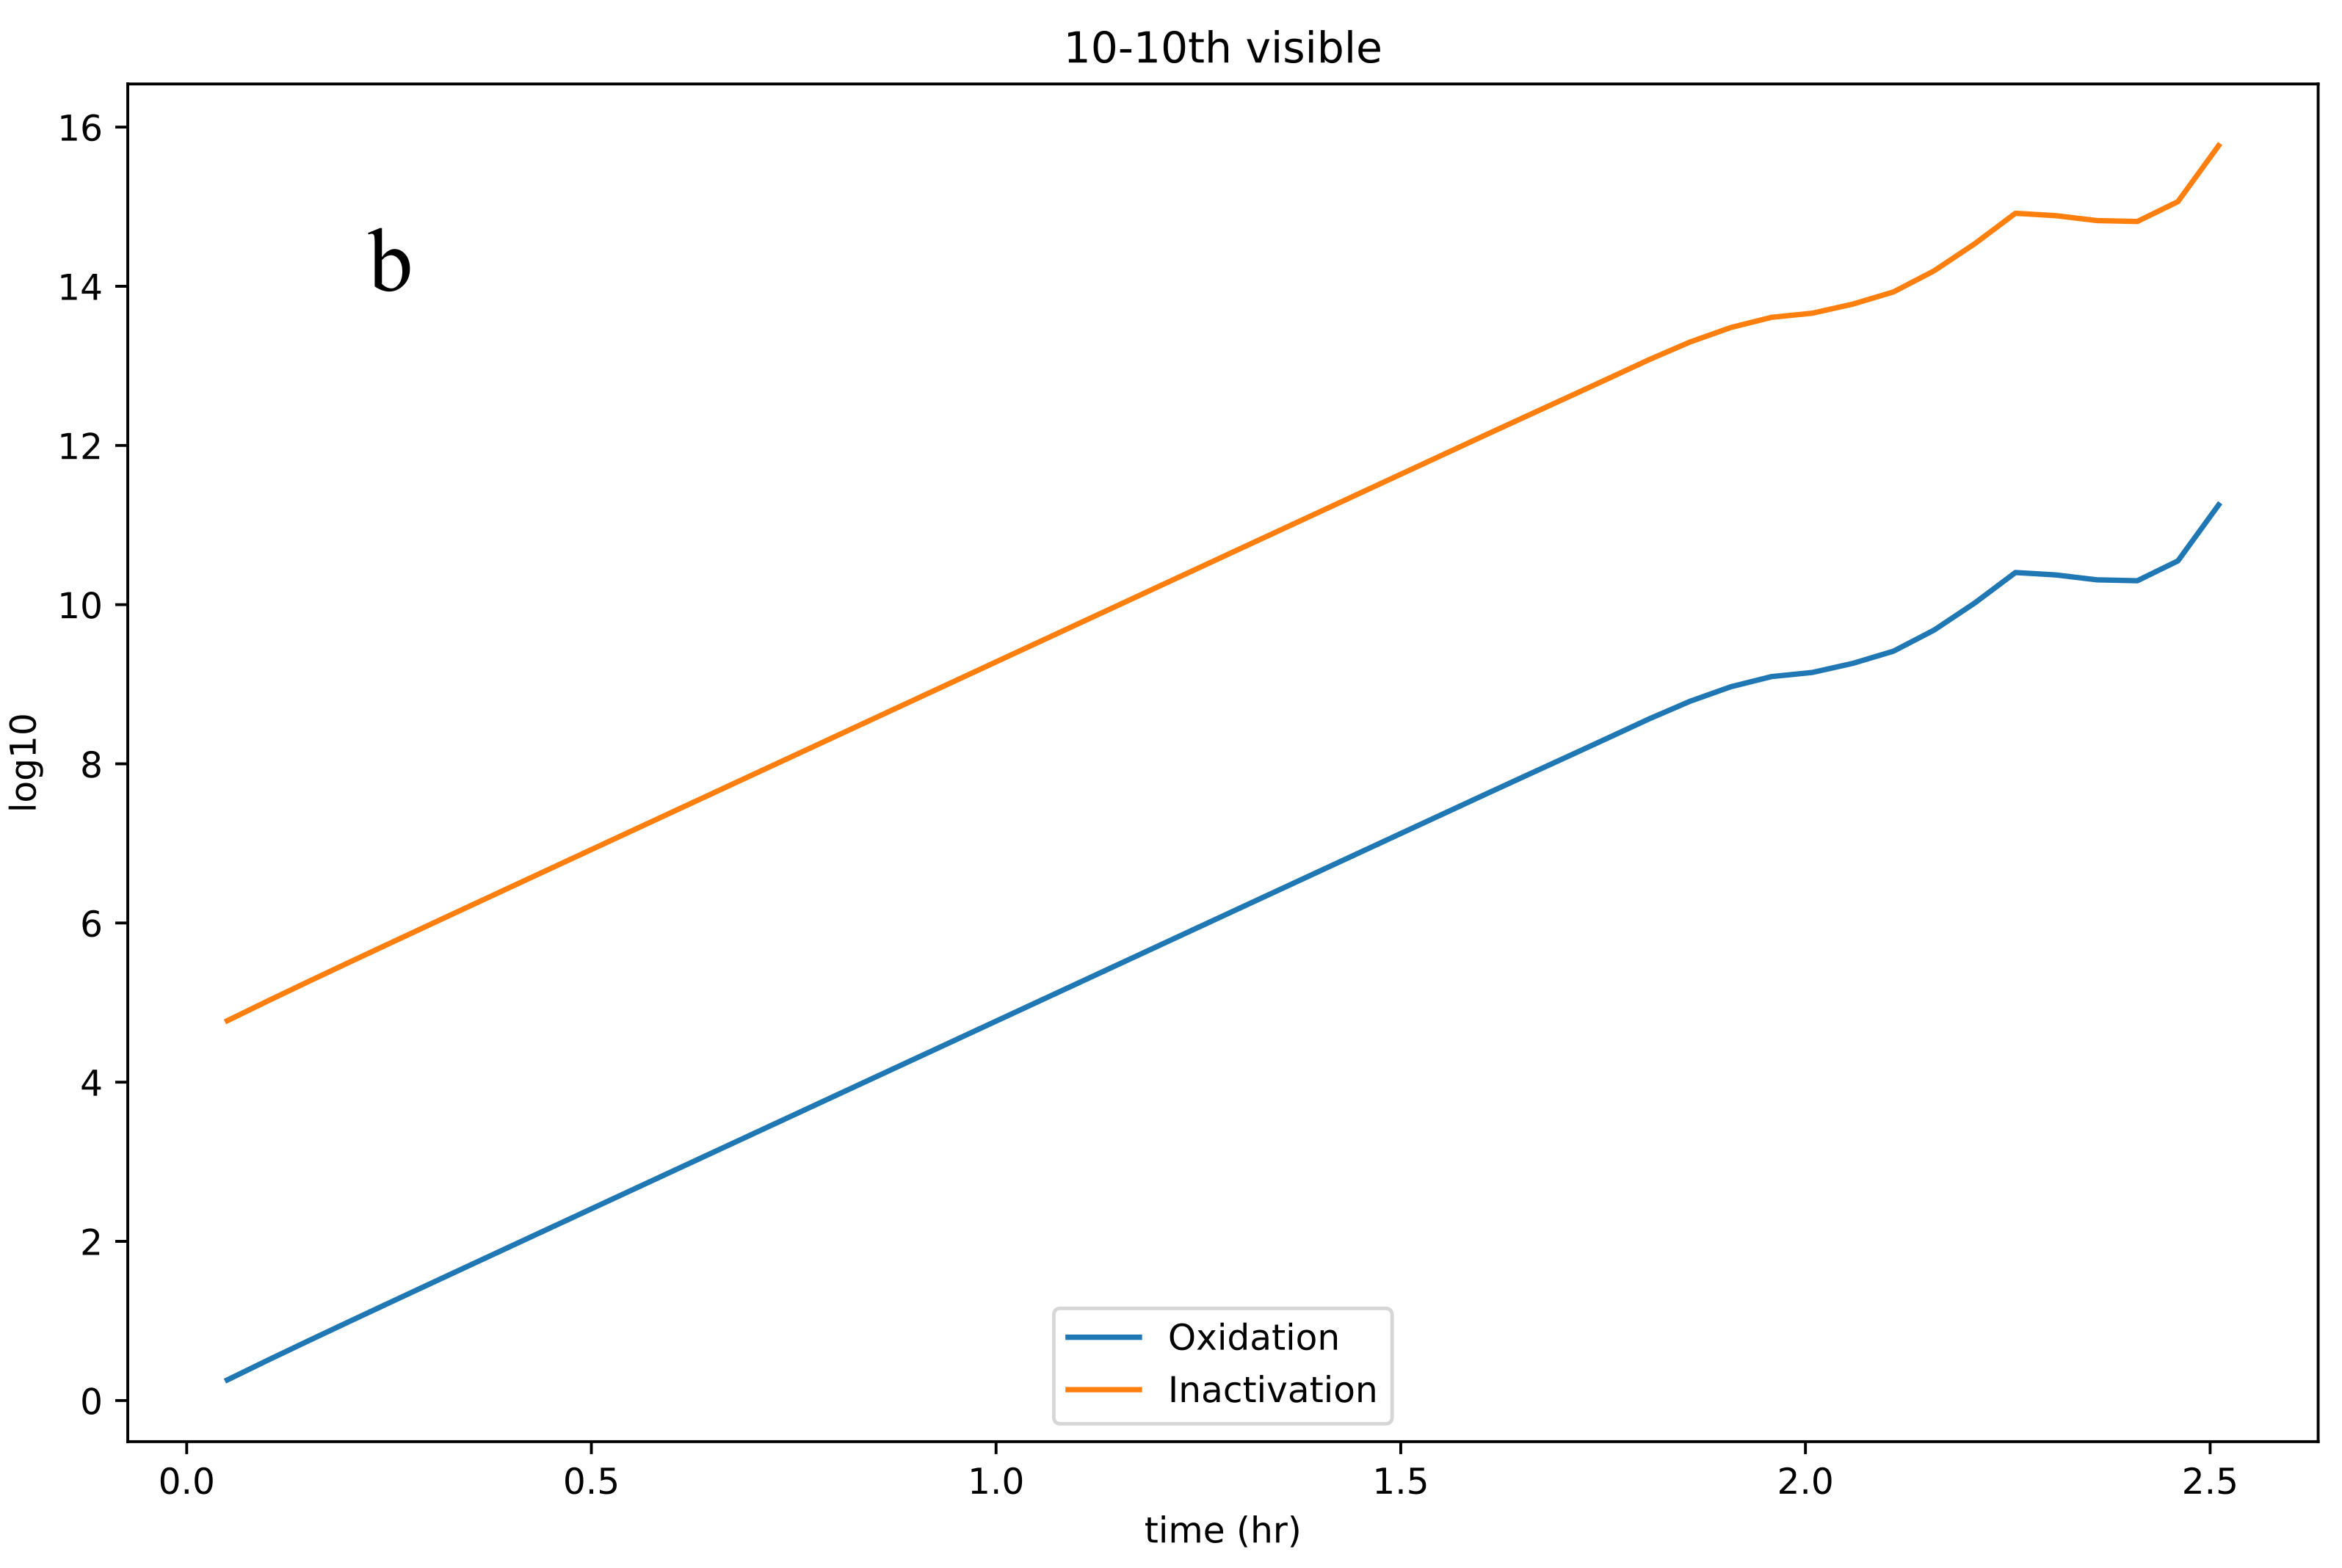
\includegraphics[width = 0.9\textwidth]{images/PDIpy/sensitivity_analyses/light_emission/100_visible.png}
    \caption{
        A comparison of the same experiment with a light source that possesses a) 20\% visible light and b) 100\% visible light, where the former value appears -- for these simulation conditions -- to be the threshold beyond which the proportion of visible light does not substantial effect inactivation rates. This threshold is likely dependent upon the quantity of incident watts; in which case, this threshold is not broadly generaliazable for all simulation conditions.
    }
    \label{light_emission}
\end{figure}

\paragraph{Bacterial CFU/mL}
The influence of bacterial $\frac{CFU}{mL}$ upon the rate of oxidation in PDIpy was tuned to yield the trend that is depicted in Figure \ref{bacterial_cfus}, where the rate of oxidation is inversely proportional with the $\frac{CFU}{mL}$. This is intuitive, where larger bacterial populations requires more time to eradicate.

\begin{figure}
    \centering
    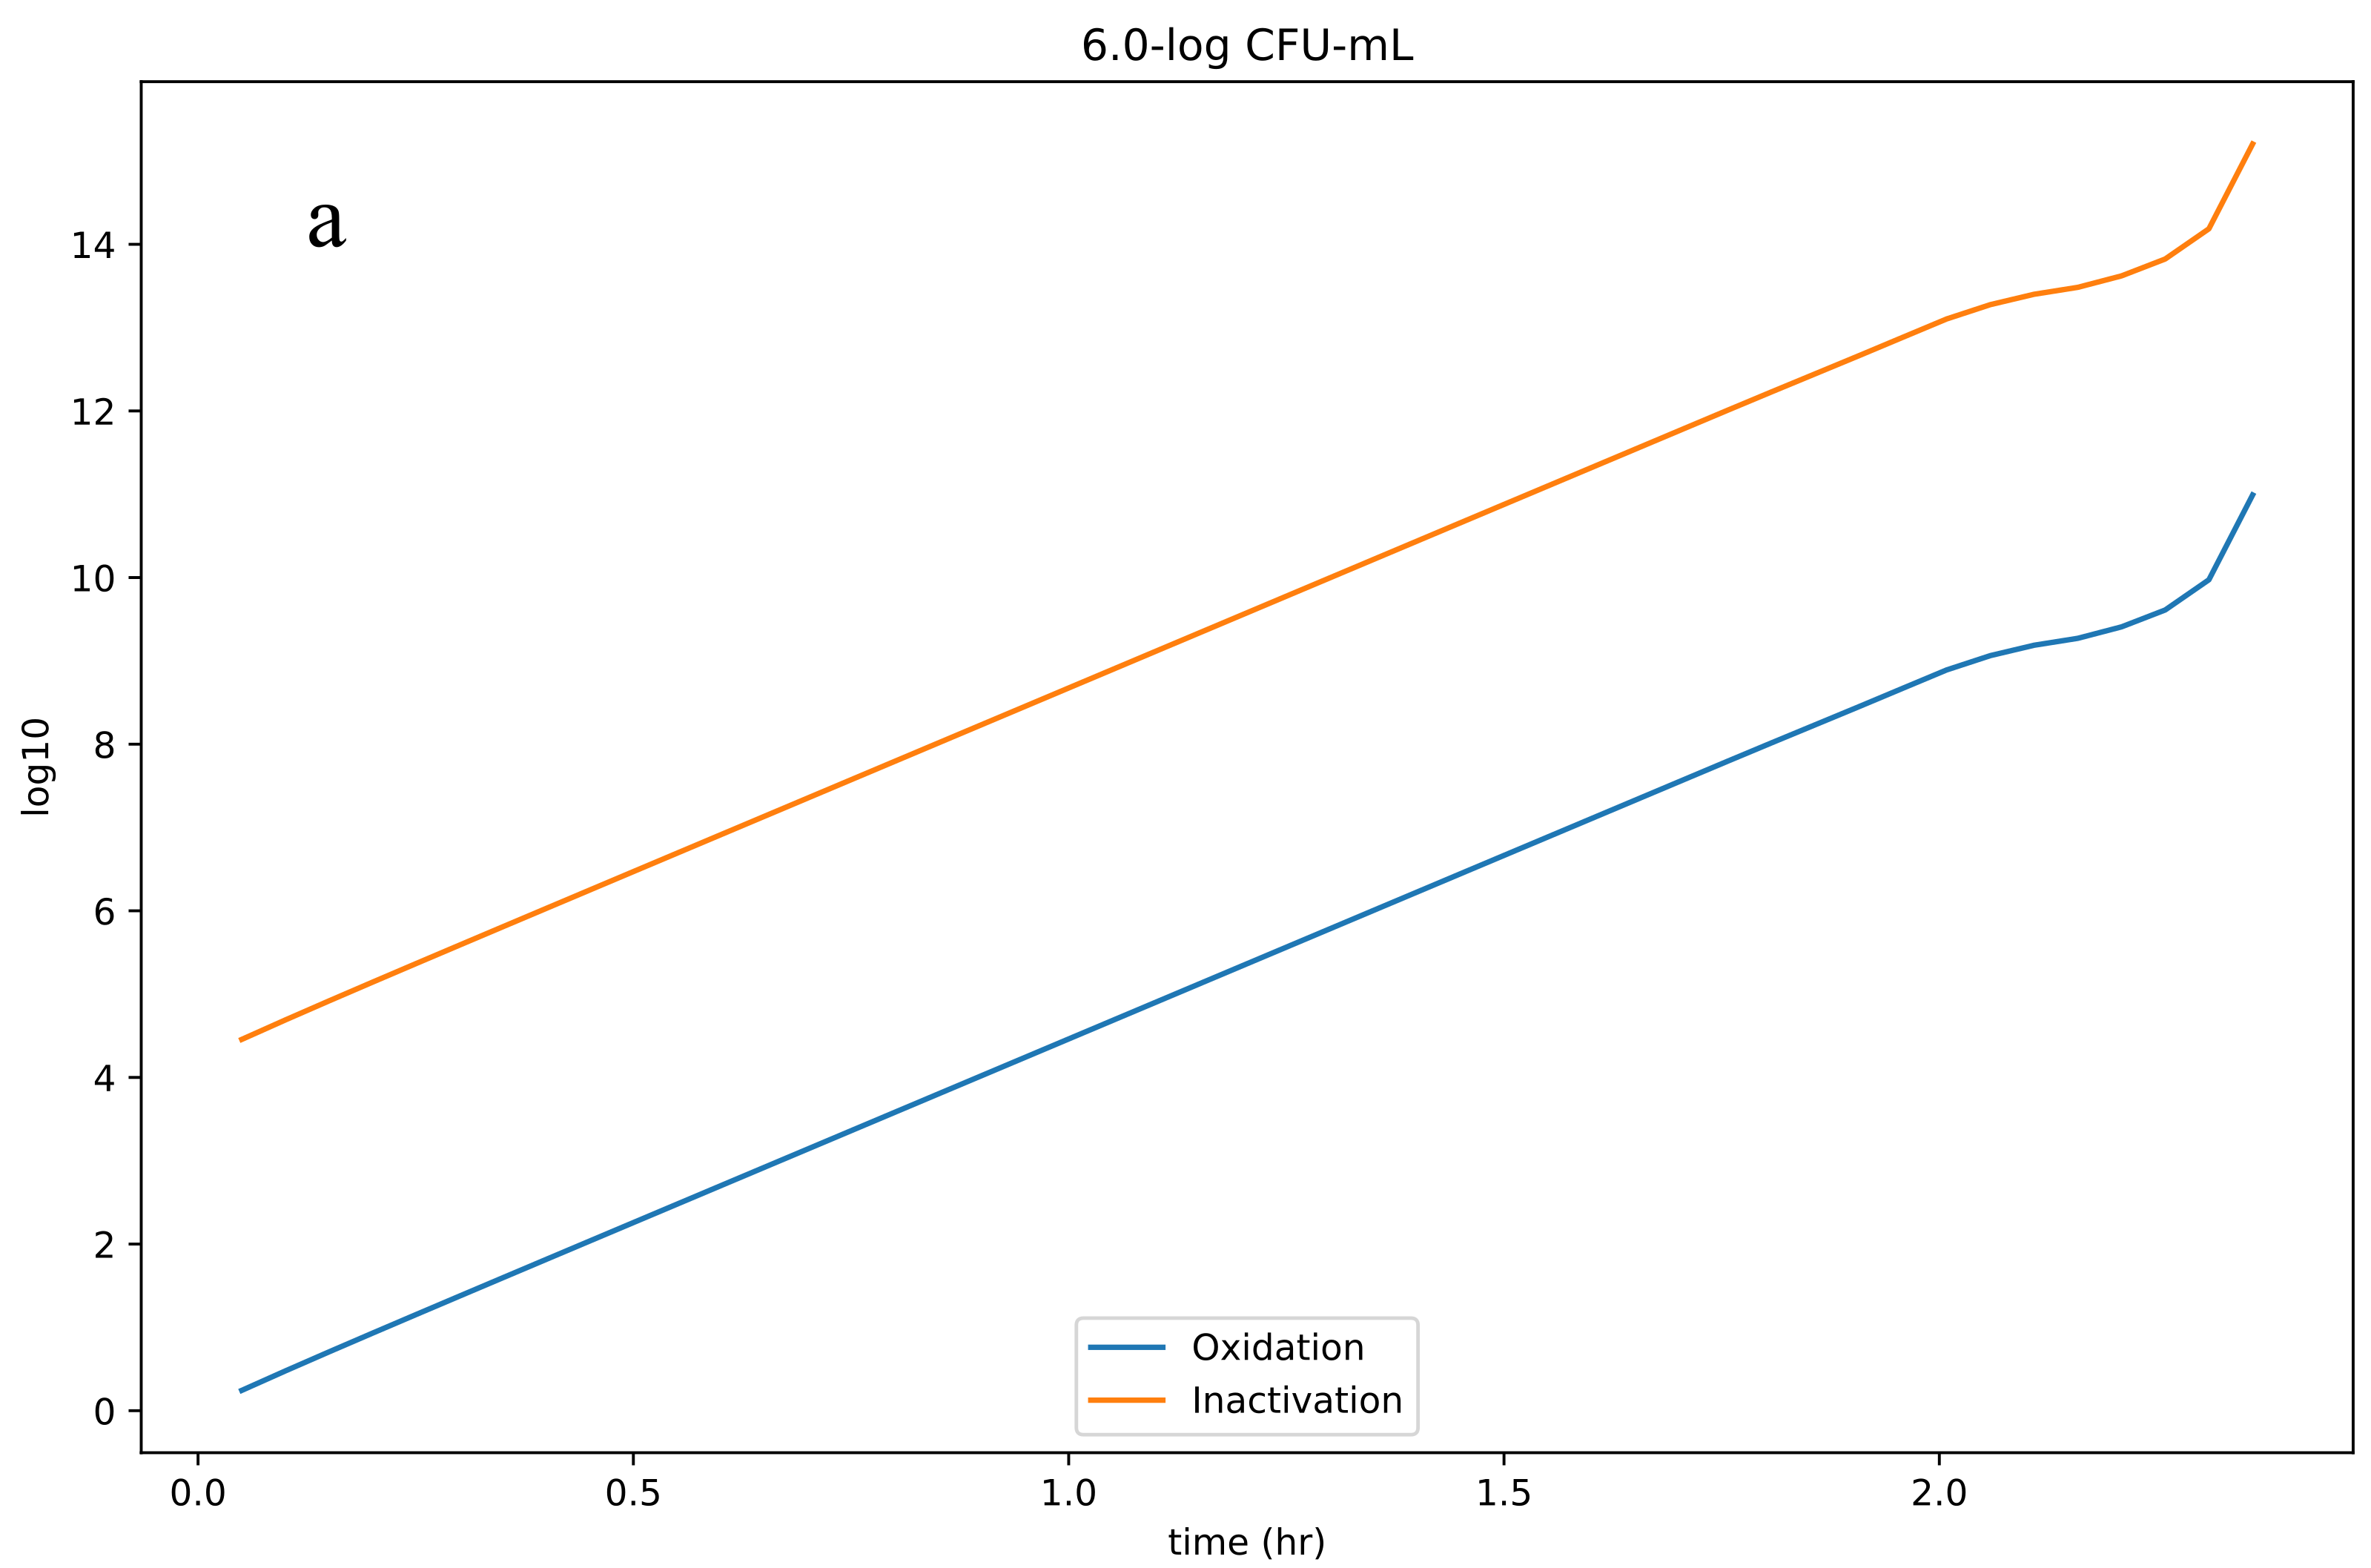
\includegraphics[width = 0.9\textwidth]{images/PDIpy/sensitivity_analyses/bacterial_cfus/6-log_cfu.png} \\
    \vspace{5mm}
    \midrule
    \vspace{5mm}
    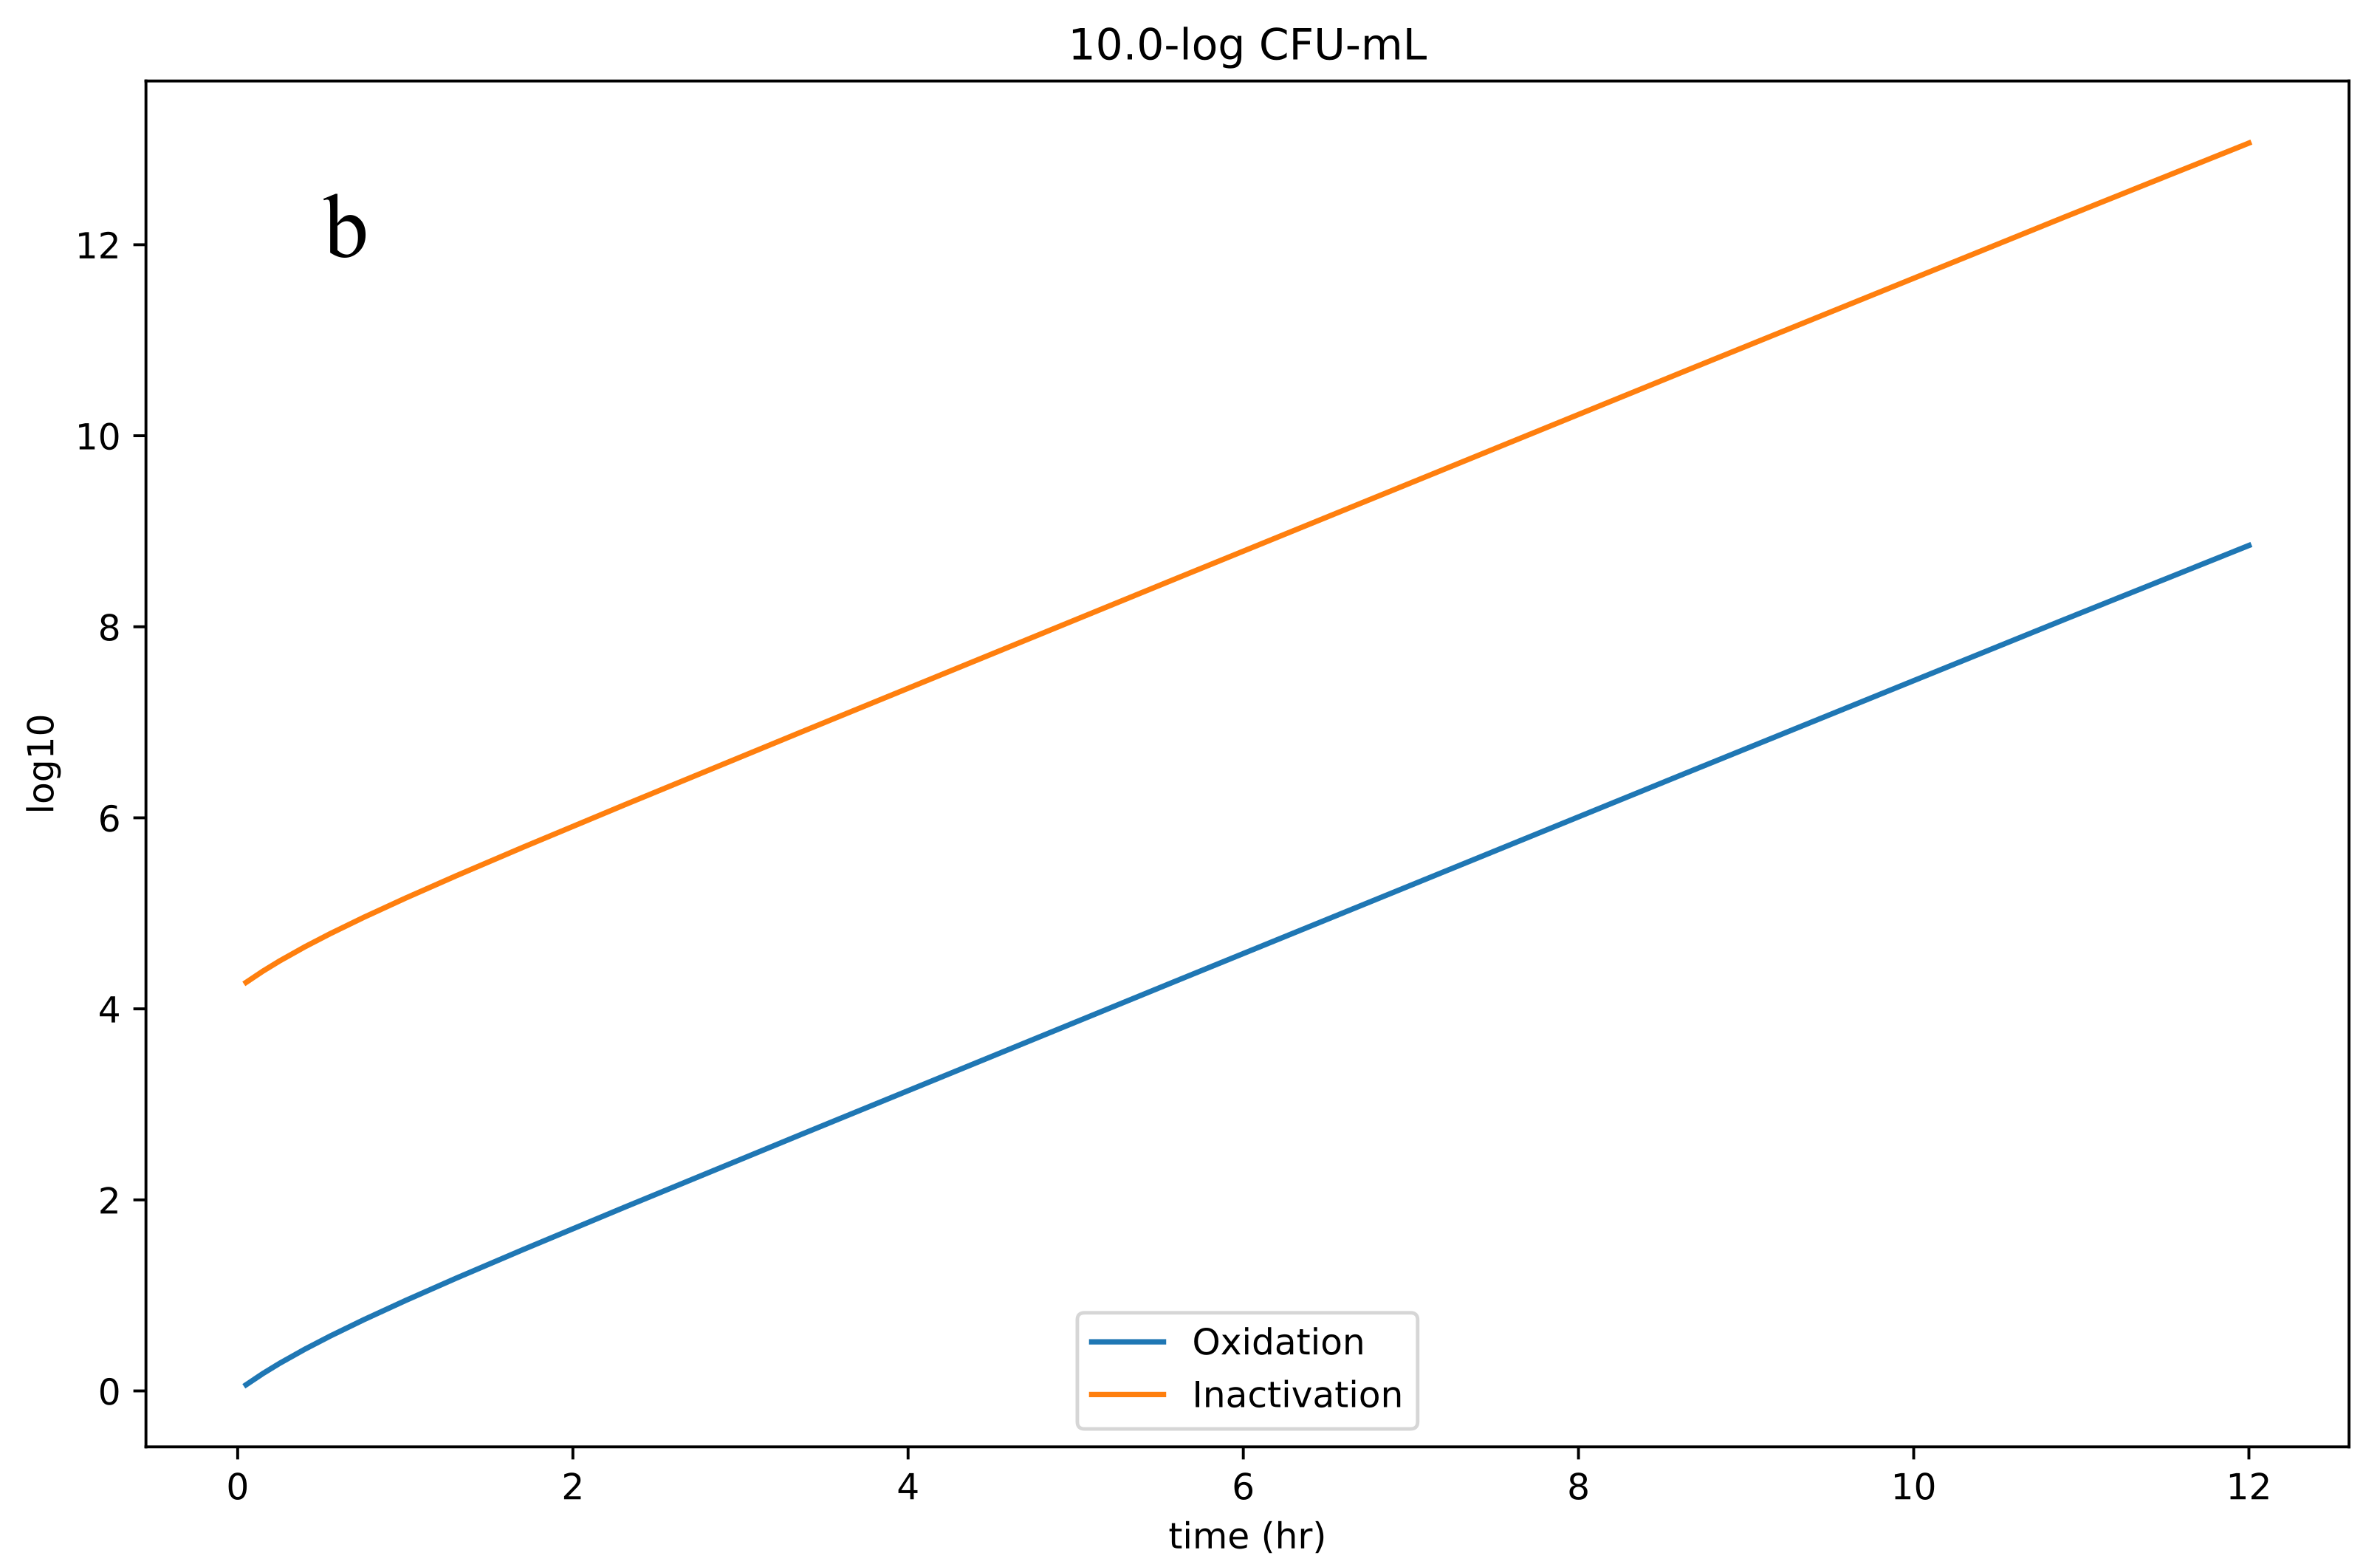
\includegraphics[width = 0.9\textwidth]{images/PDIpy/sensitivity_analyses/bacterial_cfus/10-log_cfu.png}
    \caption{
        A comparison of oxidation and inactivation between a) 1E6 and b) 1E10 $\frac{CFU}{mL}$. The imposed trend is that oxidation and thus inactivation are inversely proportional to the colony size, which is the intuitive result.
    }
    \label{bacterial_cfus}
\end{figure}

\paragraph{Photobleaching constant}
The influence of photobleaching constant was explored over an 8-log range of values, which is depicted in Figure \ref{photosensitizing_constant}. The values below $1E4$ are indistinguishable over time. 

\begin{figure}
    \centering
    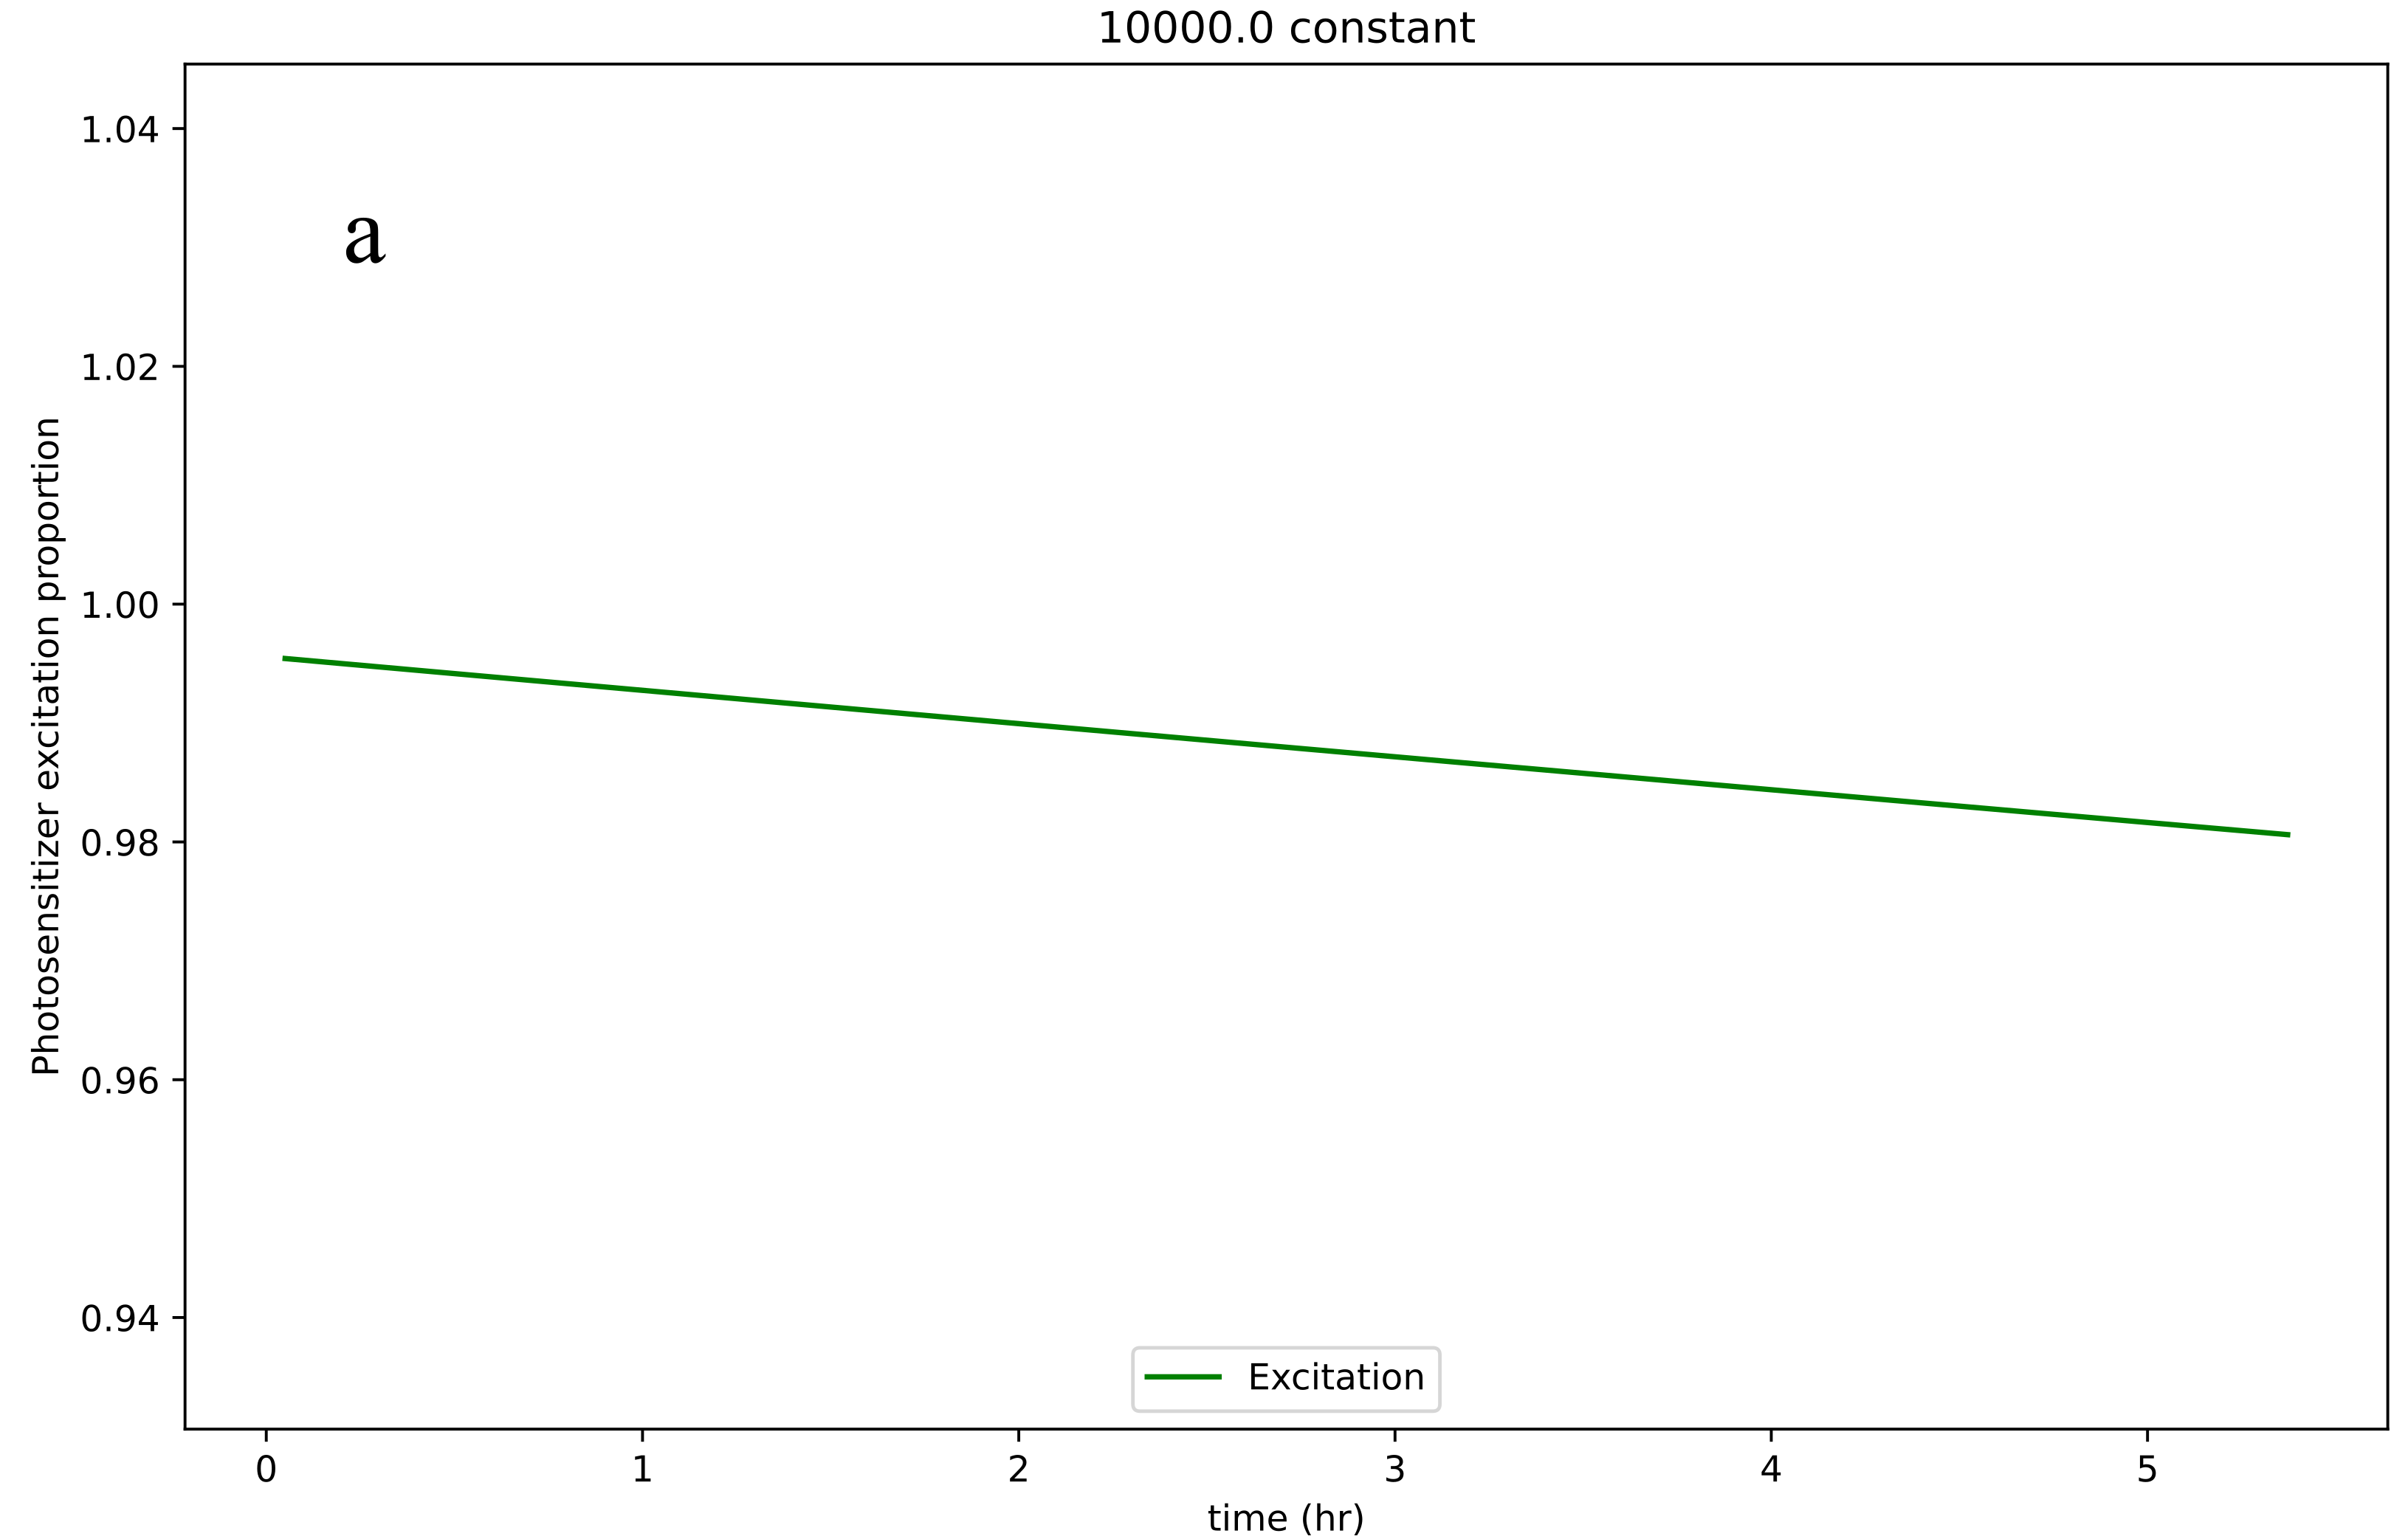
\includegraphics[width = 0.9\textwidth]{images/PDIpy/sensitivity_analyses/photobleaching_constant/1E4.png} \\
    \vspace{5mm}
    \midrule
    \vspace{5mm}
    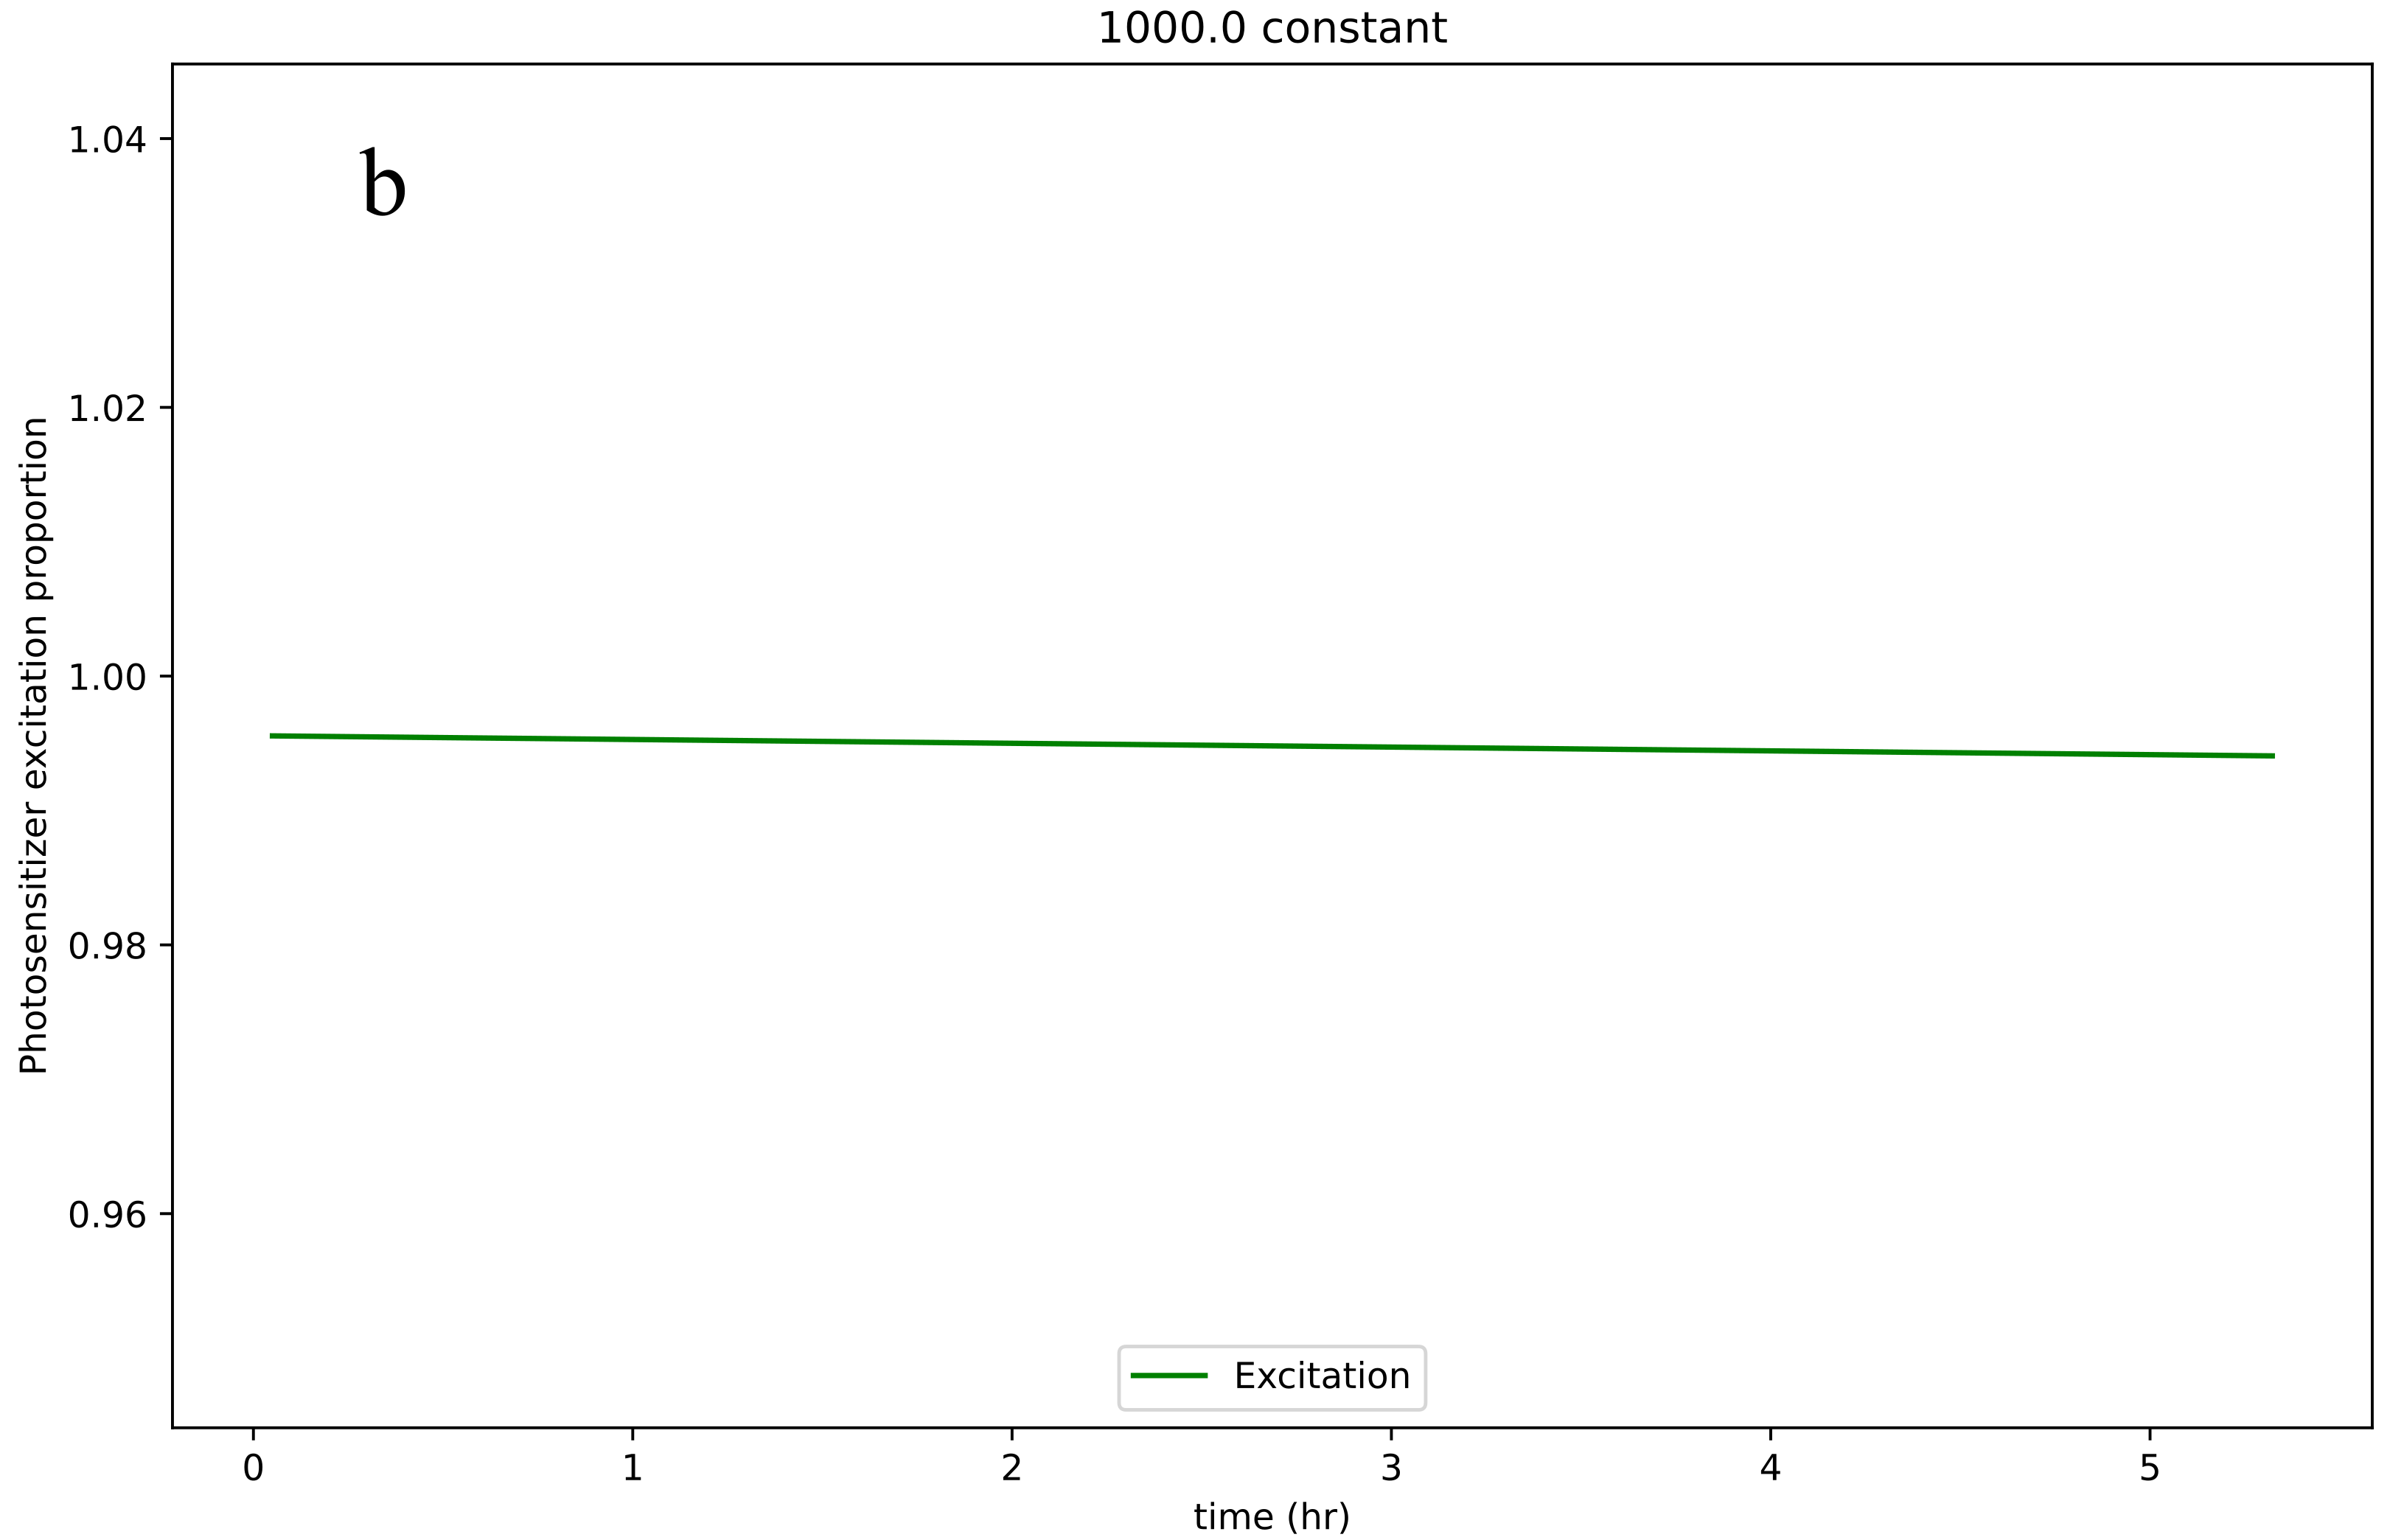
\includegraphics[width = 0.9\textwidth]{images/PDIpy/sensitivity_analyses/photobleaching_constant/1E3.png}
    \caption{
        A comparison of the excitation proportion with two photobleaching constants. Constant values below 1E4 are approximately indistinguishable.
    }
    \label{photosensitizing_constant}
\end{figure}


\subsection{Supplementary figures}
This section includes supplementary figures for the main text. The natural and synthetic porphyrins that inspire the design of photosensitizers are depicted in Figure \ref{zinc_porphyrin}. 

\begin{figure}
    \centering
    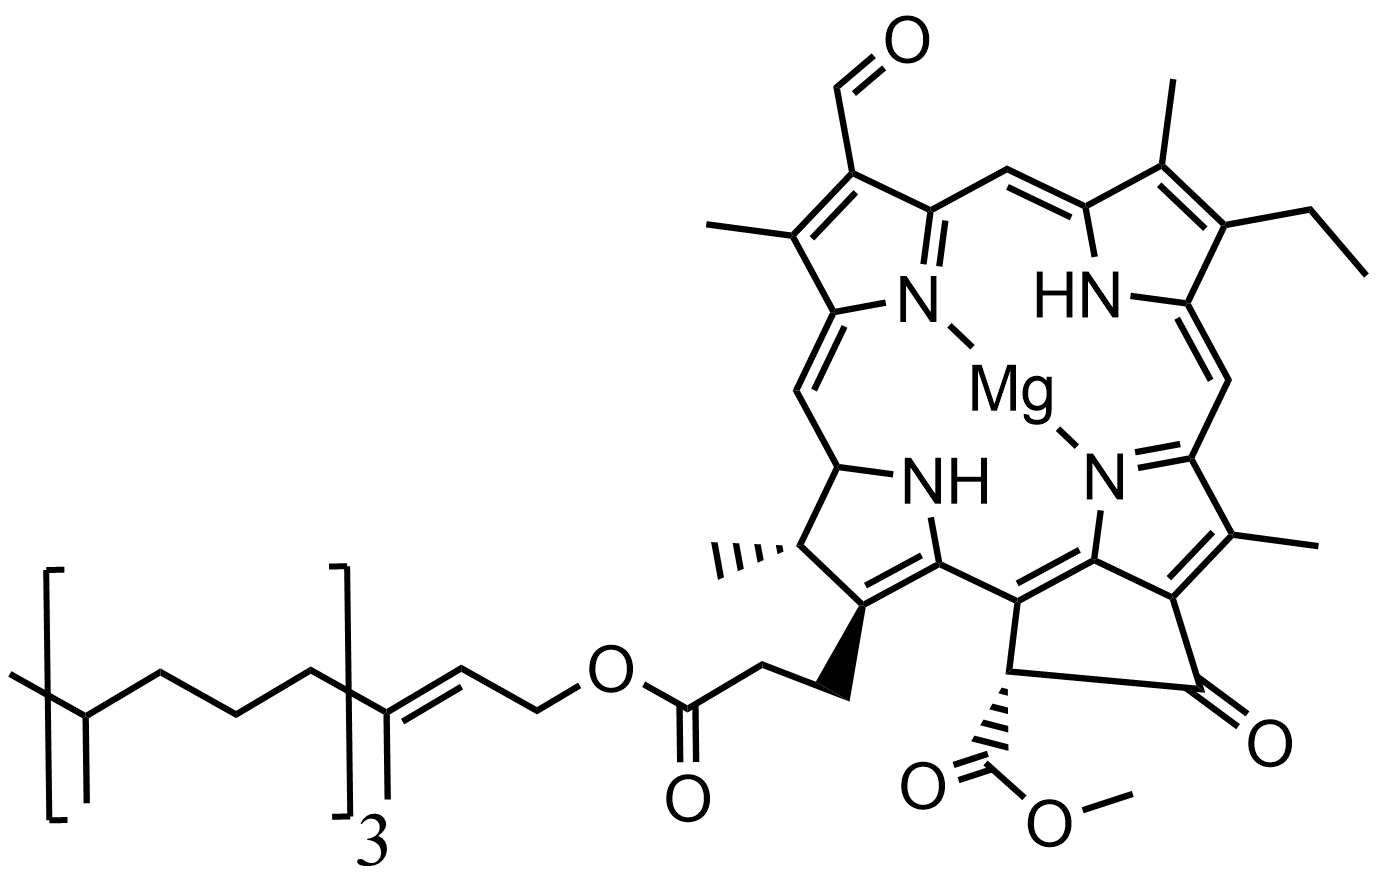
\includegraphics[width = \textwidth]{images/PDIpy/background/chlorophyll.png} \\
    \midrule
    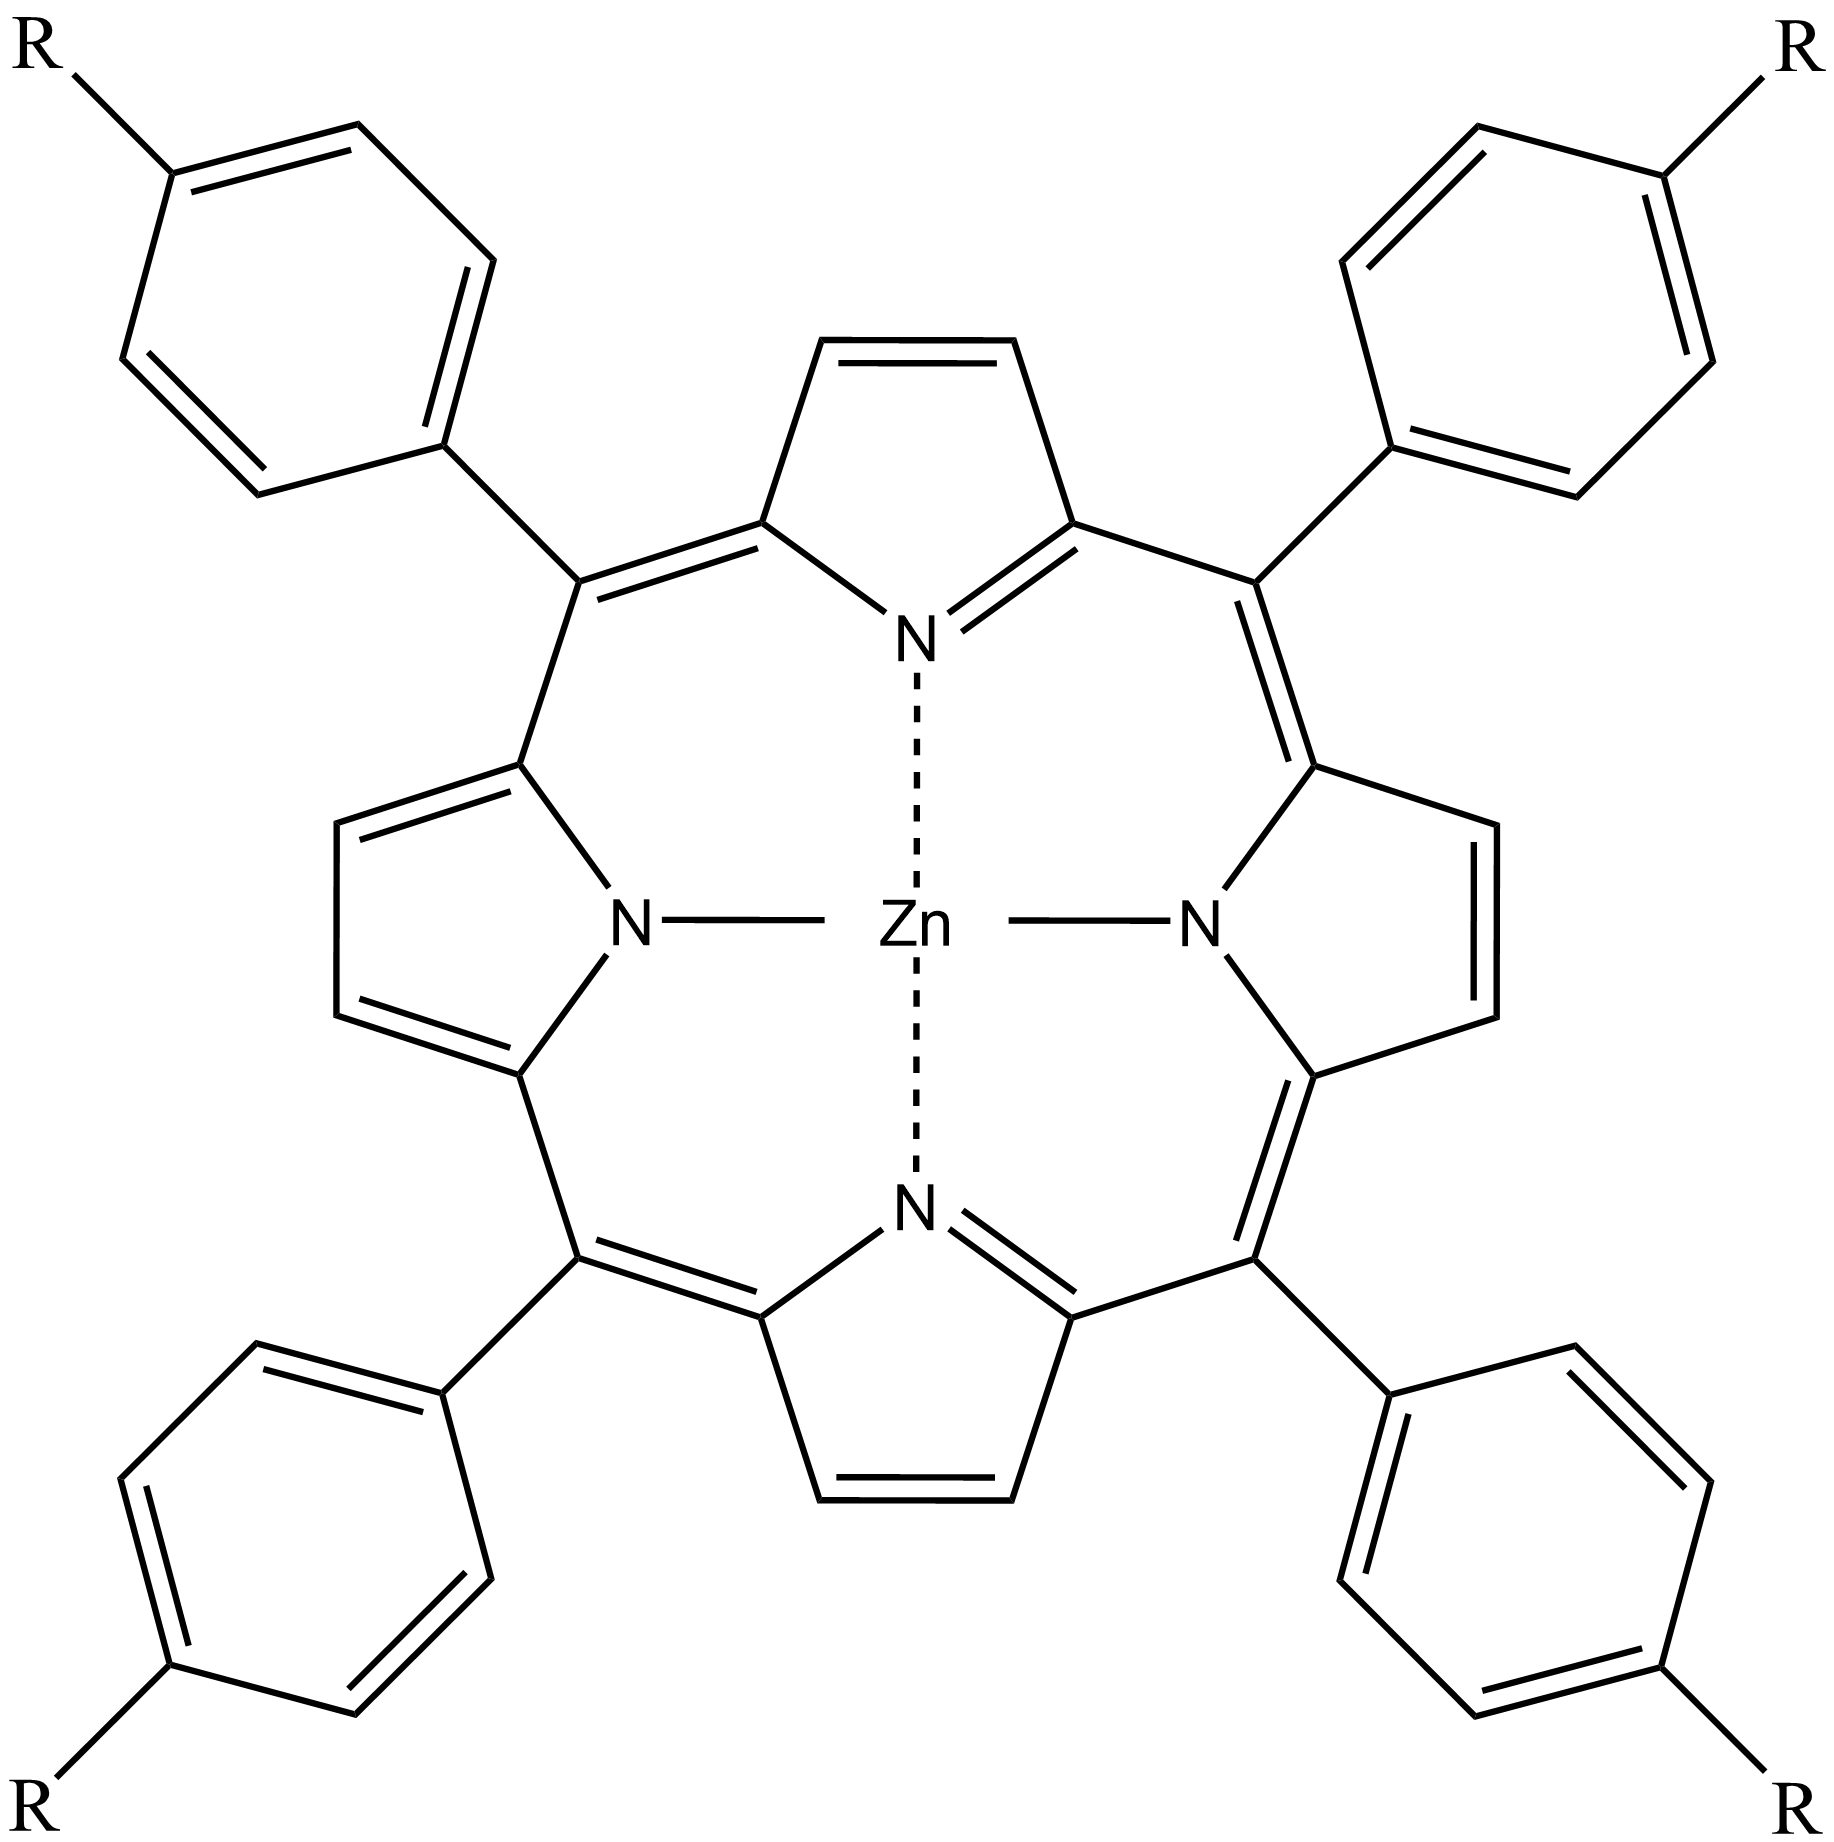
\includegraphics[width = 0.5\textwidth]{images/PDIpy/background/zinc_porphyrin.png}
    \caption{
        The chemical structure of porphyrinoid chlorophyll (top) juxtaposed with the core motif of a synthetic porphyrin analogue (bottom). The "R" groups of the synthetic porphyrin can be substituted with a range of functionality to tailor the PS for the specific PDI system.
    }
    \label{zinc_porphyrin}
\end{figure}